\documentclass[12pt]{article}
 \usepackage[hcentering,bindingoffset=20mm]{geometry}
 \usepackage{placeins}
 \usepackage[numbib]{tocbibind}
 \usepackage{rotating}
\usepackage[square,sort,comma,numbers]{natbib}
 \usepackage{graphicx}
 \usepackage{tabularx}
 \linespread{1.3}
 \usepackage{gensymb}
\usepackage{longtable}
 \usepackage{lscape}
 \usepackage{url}
 \addtolength{\textwidth}{2cm}
 \addtolength{\hoffset}{-1cm}
 
 
 \addtolength{\textheight}{2cm}
 \addtolength{\voffset}{-1cm}
 \setlength{\parindent}{0pt}
 
\title{Trial by phylogenetics - how model and data selection impacts the elucidation of the gonyaulacales (Dinophyceae). $^{1}$}
\author{Key words: Bayesian inference, model selection, gonyaulacales, phylogenetics, transcriptomics}
\date{}

\begin{document}
\maketitle
\paragraph{}Anna Liza Kretzschmar$^{2}$\\
Climate Change Cluster (C3), University of Technology Sydney, Ultimo, 2007 NSW, Australia, anna.kretzschmar@uts.edu.au
\paragraph{}Aaron E. Darling \\
The ithree institute, University of Technology Sydney, Ultimo, 2007 NSW, Australia
\paragraph{}Mathieu Fourment \\
The ithree institute, University of Technology Sydney, Ultimo, 2007 NSW, Australia
\paragraph{}Arjun Verma\\
Climate Change Cluster (C3), University of Technology Sydney, Ultimo, 2007 NSW, Australia
\paragraph{}Shauna Murray\\ 
Climate Change Cluster (C3), University of Technology Sydney, Ultimo, 2007 NSW, Australia
\newpage
\section{Abstract}
\newpage

\section{Introduction}
%TODO new direction of paper - model and data impact on phylogenetics. need to re-write intro

%good refs re systematics
%\cite{posada2016phylogenomics} start of special issue discussing systematics. Overview of problems and gold mine of references

%bullshit refs
%Galtier 08 Dealing with incongruence in phylogenomic analyses : argues against validity of ILS and for natural seletion but using morphology for being the reason why they 'can't be extensive problem in reality'. bacteria only though, doesn't hold this up for vertebrates etc.

%for later:
% fern transcriptome database, rife w paralogy www.onekp.com Rothfels '13 Transcriptome-Mining for Single-Copy Nuclear Markers in Ferns .. but use ML
For most of the history of the field of phylogenetics, the limiting factor was availability of data to infer evolutionary relationships.
Now, the breadth of publicly available in genetic information through next-gen sequencing techniques has allowed for an increasingly complex investigation into the evolutionary relationships between organisms. 
The quest for untangling these relationships is an ongoing process that can help inform a broad range of fields, including epidemiology, toxicology and trophic interactions \cite{mctavish2017and}. %TODO need more refs
The limiting factor now becomes possible errors in the methodology and understanding of the model selection underlying the phylogenetic inference by the operator.
%Taken out/re-written the following comments to change focus of manuscript:
%Advances in sequencing capabilities, computational resources and xxx have seen the use of increasing gene sets and complexity in model selection to inform phylogenetic inference. 
%The decrease in next-gen sequencing technology cost has helped make seq more common - which means that public databases of non-model organism genomes or transcriptomes are getting more betterer (fuck me I word good).
%\cite{yang2014orthology} orthologue extr method which means good discussion on problems with wrong selection
%\cite{degnan2009gene} some bullshit bout paralogs in soy bean
%Phylogenetics assessing large gene sets is becoming common practice.
%The availability of large datasets and breadth of information contained therein is phenomenal. 
%Predominantly the focus is on model organisms, however there has been a concerted effort to push non-model organisms to catch up recently. 
An example is the MMETSP project, sequencing the transcriptomes of over 650 marine eukaryotic microbes \cite{keeling2014marine}. 
This project has unlocked an unprecedented wealth of information to investigate the phylogenetics of some rather prolific branches of the tree of life. 
Here we seek to bridge some of the gap between the theoretical in computational biology and the environmental biologists exploring these types of datasets.
%However, wealth of data alone isn't sufficient for an adequate approximation of the evolution of these organisms - robust methodology is key. 
For phylogenetic inference, the gene representative for each taxa is compared with all other representatives, with the assumption of a shared evolutionary history, i.e. orthology, from which the species evolution is inferred \cite{maddison1997gene}. 
%TODO I think I jumped the gun here a little with the next sentence - explain why there can be an error
Increasing the number of genes used for inferring the species evolution can address any random sampling error, however systematic error(s) can be exacerbated by dataset increase. 
To confound this error, it can return robust support values for the incorrect phylogenetic tree inferred and obfuscate the error inherent in the analysis (see Box 1) \cite{jeffroy2006phylogenomics,roch2015likelihood,kubatko2007inconsistency}. 
Frequent issues for species tree inference arise from:\\
1) Selection of paralogs. 
If genes with different evolutionary histories are selected, the gene tree will not reflect the history of either paralog and be nonsensical for species tree inference; \\
2) Concatenation of genes. 
Can be statistically inconsistent estimator of the species tree due to incomplete lineage sorting and concatenation acting as imperfect estimator of species tree topology \cite{roch2015likelihood}; and \\
3) Inference of model adequacy from bootstrap values. 
Kubatko et al. (2007) demonstrated high bootstrap support under maximum likelihood (ML) inference for incorrect species trees with concatenated gene sets as input \cite{kubatko2007inconsistency}. 
As high bootstrap values are often used as an indicator for robust species topology resolution, this fallacy is particularly problematic if the reader/operator is unfamiliar with the statistical phenomenon (see box 1 for).\\
In this study we aim to demonstrate a bioinformatic methodology which is more robust to paralogy when processing transcriptomic data than currently commonly utilized in protistology. 
Further, we seek to demonstrate the impact of model and data selection on the resulting phylogenetic inference. 
Specifically, the scripts available with this study assemble RNA-seq datasets, identifies and extracts single copy genes across input taxa with extensive paralogy, and runs Bayesian inference (BI) phylogenetics. 
Finally, a comparison between commonly used phylogenetic methods to the historically difficult order Gonyaulacales (phylum: Dinoflagellata) which are notorious for the issues that this study seeks to draw attention to (see box 2 for further information on the gonaylacales).\\

%TODO need to bridge the gap in knowledge for taxonomists
\subsubsection*{Box 1: Statistical nomenclature \& errors this study seeks to address}
For in depth explanations see \cite{yang2014molecular}.\\
\textbf{Maximum likelihood estimate:} estimates parameters of a statistical model with maximises the parameter's likelihood function. 
Does not use priors, which means probability functions not applied to model parameters, but only their estimates. 
Model reparametrization does not affect MLE, in effect a static method.\\
\textbf{Bayesian probability:} infers posterior probability from expectation based prior probability and data based likelihood function.
BI uses probability distributions to describe uncertainty in parameters.
Model reparametrization via priors changes posterior output, i.e. a dynamic method informed by observation. 
We recommend Huelsenbeck et al. (2001) for an overview of the principles underlying BI for phylogenetics \cite{huelsenbeck2001bayesian}.\\
\textbf{Heterotachy:} change in evolutionary rates of sites over time, specific to lineage(s).\\
\textbf{Potential statistical error types:}\\
1. random. Sampling based error which decreases and approaches zero as size of dataset approaches infinity.\\
2. systematic. Arises from incorrect model assumptions or problems with the model itself. 
Error type persists and increases as dataset size approaches infinity. 
If strong, can override true phylogenetic signal.\\
\textbf{Incomplete lineage sorting:} discordance of gene evolutionary history with the species evolutionary history causing the phylogenetic species tree to be misinfered.\\
\textbf{Long branch attraction:} phylogenetic phenomenon where distantly related taxa are inferred as close relatives due to systematic error, also known as the Felsenstein zone.

\subsubsection*{Box 2: Who/what are the gonyaulacales?}
%TODO Aaron and Mathieu, as non protistologists is this section adequate in explaining why the gonyaulacales were chosen for this work, or would it help to include some of the commented out text?
The gonyaulacales are an order within the super-phylum alveolata and sub-phylum dinoflagellata, which are an ancient lineage on the eukaryotic branch of life \cite{moldowan1998biogeochemical}. 
%They play a role in several important ecological processes, as members are represented in aquatic environments, where the cover a diverse niches such as symbionts, parasites and some taxa can cause harmful algal blooms through proliferation and/or neurotoxin production \cite{murray2016unravelling}.
Dinoflagellates possess large genomes (estimated 3.7 to 220 Gbp) \cite{casabianca2017genome}, with extensive paralogy and repetitive short sequences. 
For a review on the genetic features of dinoflagellates see \cite{murray2016unravelling}. 
While the evolutionary relationship of most orders within the dinoflagellates has been inferred with consistently high support values, one order has often escaped elucidation - the gonyaulacales. 
%Analyses for this order commonly combined concatenation and maximum likelihood approaches, which yielded long branch attraction, low confidence values and inconsistent taxon resolution \cite{}. 
Improving upon the species the evolution of the gonyaulaceles has implications for environmental disease monitoring, as neurotoxin production is prevalent in this order and the direct cause of paralytic shellfish poisioning, ciguatera fish poisoning, e.g. \cite{shalchian2006combined,zhang2007three,saldarriaga2004molecular,hoppenrath2010dinoflagellate,murray2005improving}. 
%Specifically the ciguatoxins produced by some \emph{Gambierdiscus} spp. are of interest as the causative agent of ciguatera fish poisoning, a neglected tropical disease with global implications \cite{globalcig}.%, which is predicted to increase in prevalence as climate change progresses \cite{}.

\newpage
\section{Materials and methods}
\subsection*{Culture conditions}
\FloatBarrier
Cultures were isolated from locations as per Table S1 and clonal cultures established by micropipetting single cells through sterile seawater. 
Clonal cultures were maintained in F/10 medium and maintained at temperatures indicated in Table S1. 
%AD 160117: do you think these are actually clonal? Does the term clonal as used in euk microbiology include commensal bacteria? clonal but not necessarily axenic? // Yep, that's spot on - clonal but not axenic. These critters tend to die faster than a snowball in a bushfire without their bacteria

\subsection*{RNA isolation}
\emph{Gambierdiscus} spp. and \emph{Thecadinium} cf. \emph{kofoidii} were harvested during late exponential growth phase by filtration onto 5 $\mu$m SMWP Millipore membrane filter (Merck, DE) and washed off with sterile seawater. 
Cells were pelleted via centrifugation (make of centrifuge) for 10 minutes at 350 rcf. 
Supernatant was decanted and 2ml of TRI Reagent (Sigma-Aldrich, subsidiary of Merck, DE) was added to the pellet and vortexed till dissolved. 
Samples were split in two and transferred to 1.5ml eppendorf tubes. 
Cellular thecae were ruptured by three rounds of freeze-thaw, with tubes transferred between liquid Nitrogen and 95 $^{\circ}$C. 
RNA was extracted as per protocol for TRI Reagent. 
RNA elute was purified with the RNeasy RNA clean up kit EXACT NAME as per protocol(Qiagen). 
DNA was digested with TurboDNAse (Life technologies, subsidiary of Thermo Fischer scientific, AU). 
RNA was quantified with Nanodrop 2000 (Thermo Scientific, Australia) and frozen at -80 $^{\circ}$C until sequencing.
%TODO insert centrifuge, kit name deets
 
\subsection*{Library preparation and Sequencing}
The quality of samples was assessed via Agilent 2100 Bioanalyzer. 
Paired-end sequencing was performed on NextSeq 500 High Output at the Ramaciotti Centre (UNSW, AU) with 75bp insert size for \emph{G. lapillus} and \emph{G.} cf. \emph{silvae}; and 150bp inserts for \emph{G. carpenterii}, \emph{G. polynesiensis} and \emph{T.} cf. \emph{kofoidii}.

\subsubsection*{Publically available transcriptome libraries}
The \emph{Gambierdiscus excentricus} VGO790 transcriptome was downloaded from NCBI under accession ID SRR3348983 \cite{kohli2017role}. 
\textit{Coolia malayensis}, \textit{Ostreopsis ovata}, \textit{Ostreopsis rhodesae} and \textit{Ostreopsis siamensis} sequencing libraries were supplied by Arjun Verma (Verma 2018, in prep). 
RNA seq libraries for all remaining transcriptomes were generated by, and downloaded from, the Marine Microbial Eukaryote Transcriptome Sequencing Project \citep{keeling2014marine}.

\subsection*{Transcriptome processing scripts}
The scripts are packaged in the Nextflow language \cite{nextflow} for streamlined transferal between high performance computing clusters and available on Github under hydrahamster/gonya\_phylo. 
The workflow is separated into two parts, and modules within the scripts are written in bash and Python 2.7 \cite{python}, including the pandas module \cite{pandas}, and can be found on github. 
%AD 160118: do you want to give the two parts more descriptive short names? // Better ^___^ but maybe not on the short front
The scripts were executed on the Genomics Virtual Lab (GVL) \cite{afgan2015genomics}.
\subsubsection*{Scripting part 1: Transformers, assemble!}
Individual RNA sequencing libraries are the input, which are then processed through FastQC \cite{fastqc} for quality metrics, sequences are trimmed with Trimmomatic (LEADING:3 TRAILING:3 SLIDINGWINDOW:4:5 MINLEN:25) \cite{bolger2014trimmomatic} and assembled with Trinity v2.4.0 (default settings for paired end libraries) \cite{haas2013novo}. 
Assemblies were then processed with BUSCO2 with the protist specific library \cite{simao2015busco}.
The RNA libraries with 150bp inserts generated as part of this study were also subjected to Digital Normalization \cite{diginorm} prior to assembly, to pool identical transcripts before assembly.                                                                                                                                                                                                                                                                                                                                                                                                                                                                                                                                                                                                                                                                                                                                                                                                                                                                                                                                                                                                                                                                                                                                                                                                                                                                                                                                           
\subsubsection*{Scripting part 2: Klondike gold rush}
The BUSCO2 output from all transcriptomes in the previous script run is the input for the second round. 
Any genes that were present in at least 75 \% of the transcriptomes were indexed, the corresponding contig extracted from the assemblies, aligned with hmmer3.1b2 \cite{eddy2015hmmer} and unaligned regions trimmed.
If several candidate sequences are processed for the same organism, a warning message in the command interface alerts the user before proceeding. 
The output for this section was used as basis for single copy gene phylogenetic inferences in subsequent sections.

\subsection*{Assembly analysis}
Contigs from assemblies were clustered with cd-hit with the flaps T 10 -M 5000 -G 0 -c 1.00 -aS 1.00 -aL 0.005 \cite{fu2012cd}. 
Protein coding regions were predicted with Transdecoder \cite{haas2016transdecoder}.
Amino acid clusters were clustered again with cd-hit with the flags as previously except -c 0.98.
Protein sequences were analysed with interproscan v5.27 with local lookup server \cite{quevillon2005interproscan}.

\subsection*{Phylogenetic inferences}
\subsubsection*{rDNA based inference}
\paragraph*{Maximum likelihood with concatenated sequences.}
\paragraph*{Bayesian probability with concatenated sequences.}
Ribosomal DNA sequences for the small subunit region as well as the D1-D3 large subunit region were acquired from NCBI \cite{coordinators2017database} or the SILVA rRNA database project \cite{silvaproj}, accession IDs in Table S3. 
Individual genes were aligned using the MUSCLE algorithm a maximum of 8 iterations \cite{edgar2004muscle}, then were concatenated in Geneious v11.3 \cite{kearse2012geneious}.
ML inference was obtained using RaxML \cite{stamatakis2014raxml} with the GTR and GAMMA flags, with 100 bootstraps.

\subsubsection*{Single copy gene based inference}
\paragraph*{Maximum likelihood with concatenated sequences.}
\paragraph*{Bayesian probability with concatenated sequences.}
Sequences were concatenated and ML inference run as described in the previous section, with the ILGF, GAMMA and PROT flags.
BI was run in BEAST2 with the Gamma site model with 4 Gamma category counts under the WAG amino acid model. A local random clock was used  under the Birth Death model %TODO MATHIEU what was the end nuber of chains?
Both ML and BI inferences were run the HPCC. 

\paragraph*{Bayesian probability under multispecies coalescence.}
Subsequent analyses were executed on the University of Technology Sydney's High-performance computing cluster (HPCC).
%AD 160118: the P in HPC is for performance - not power, though neither adjective is very appropriate for UTS's cluster :( // true that
Species evolutionary inference was based on BI with the *BEAST2 model in BEAST2 \cite{bouckaert2014beast}. 
%TODO make a sensical something as 'Bayesian probability'
The analysis was performed under the WAG substitution model \cite{whelan2001general} with a Gamma distribution for four rate categories. 
A random local clock was employed \cite{drummond2010bayesian}.
Posterior distributions of parameters were approximated after 300,000,000 generations of MCMC runs with 4 heated and one cold chain, sampled every 5,000 generations  with a burn in of 15\%. 
The inference was run four times to compare convergence of parameters, then log and tree files were merged. 
Inference was accelerated using BEAGLE \cite{ayres2011beagle} on the GPU.

\subsection*{Path sampling}
%TODO Mathieu please put details in

\subsection*{Inference run time comparison}
A subset of 14 taxa was selected for a comparison between CPU and GPU inference run time comparison. 
The transcriptome libraries were fed through the single copy gene extracrion script as described, which was set to extract single copy genes present in all of the taxa. 
The resulting alignments were run on *BEAST either on the CPU or GPU.

\subsubsection*{Generation of figures}
Tanglegrams were generated with Dendroscope v3.5.9 \cite{huson2007dendroscope}; images were edited in GIMP \cite{gimp}.
\newpage
\section{Results}
\subsection*{Transcriptomes overview}
RNA-sequencing libraries are available on NCBI's sequence read archive under SRP134273.
Sequencing of transcriptomes for \emph{Gambierdiscus} spp. and \emph{T.} cf. \emph{kofoidii} generated datasets ranging in size from, 143,155,667 to 233,822,334 reads, resulting in 97,634 to 191,224 assembled contigs (table ~\ref{tbl:asmstats}). 
Approximately XX\% to XX\% predicted to be protein coding sequences. 
%TODO Interpro scan, SRA IDs
\FloatBarrier
\begin{longtable}{  | p{3cm} |p{2.2cm} | p{2.2cm} | p{2.2cm} | p{2.2cm} | p{2.2cm} |}
\caption{Summary of transcriptome sequencing and assembly statistics.}\\
\hline
\label{tbl:asmstats}
\emph{Sequences:}&\emph{G. carpenteri}&\emph{G. lapillus}&\emph{G. polynesiensis}&\emph{G.} cf. \emph{silvae}&\emph{T.} cf. \emph{kofoidii}\\
\hline
 \multicolumn{6}{| c |}{Sequencing}\\
 \hline
\textbf{SRA accession}&SRR6821720&SRR6821722&SRR6821723&SRR6821721&SRR6821724\\
\hline
\textbf{Raw sequencing reads}&186,422,744&145,366,966&217,031,342&143,155,667&233,822,334\\
\hline
%\textbf{Size (Gb)}&16.92&&19.51&&21.08\\
%\hline
 \multicolumn{6}{| c |}{Assembly}\\
 \hline
 \textbf{Contigs \#}&105,464&148,972&114,622&191,224&97,634\\
\hline
\textbf{Average length (bp)}&607&1,139&633&953&581\\
%\hline
%\textbf{Minimum length (bp)}&201&201&201&201&201\\
\hline
\textbf{Maximum length (bp)}&7,448&12,370&6,608&8,198&7,922\\
\hline
  \multicolumn{6}{| c |}{Transcript clustering \& annotation}\\
\hline
\textbf{\# clusters}&139,699&92,418&139,487&107,766&116,468\\
\hline
\textbf{with protein functional domains}&&&&&\\
\hline
%\textbf{with full annotations}&&&&&\\
%\hline
%\textbf{with Enzyme Codes}&&&&&\\
%\hline
%\textbf{mapped to KEGG pathways}&&&&&\\
%\hline
\end{longtable}

\subsection*{BUSCO output}
Assemblies for all transcriptome datasets used in this study were searched with BUSCOv2 and single copy genes extracted. 
The single copy genes acquired though the BUSCO hmmer libraries curated for protists are reported in Table S2 out of the total 234 genes searched for, as well as accession numbers and identifiers for each transcriptome. 
Single copy genes for each transcriptome used in this study are available on Zenodo DOI:
%TODO single copy genes need ot go up on Zenodo, then link DOI here

\subsection*{Phylogenetic inferences}
Support for branches was interpreted as follows, for ML and BI, respectively: 100\%/1.0 was considered fully supported, above 90\%/0.9 was very well supported, 80\%/0.8 and above was interpreted as relatively well supported and above 50\%/0.5 was considered supported but below was considered unsupported.
As \emph{Azadinium spinosum}, \emph{Dinophysis acuminata} and \emph{Karenia brevis} are considered the outgroup to this study, the unifying branch for these taxa was used to root the tree in all subsequent analyses.
\subsubsection*{rDNA based phylogeny}
\FloatBarrier 
All nodes were supported, with a range of certainty (Fig. ~\ref{fig:rdna}).
Species with the genera \emph{Gambierdiscus} and \emph{Ostreopsis} resolved with their sister species with full support. 
Within the \emph{Gambierdiscus} clade, nodes are either supported or fully supported. 
The two species of \emph{Alexandrium} resolve as well supported closest relatives, but do not form an individual clade. 
Deeper nodes were supported but with less certainty than the crown taxa. 
Two distinct clades can be observed from the topology: One including \emph{Alexandrium}, \emph{Coolia} and \emph{Ostreopsis}; another with only \emph{Gambierdiscus}. 
Sister to these clades, in descending order, was \emph{Pyrodinium}, \emph{Ceratium} and \emph{Gonaulax}, \emph{Protoceratium} and \emph{Thecadinium}. 
The outgroup was relatively well supported and included \emph{Crypthecodinium}. 
Support for deeper nodes varied from supported to well supported.

\begin{figure} 
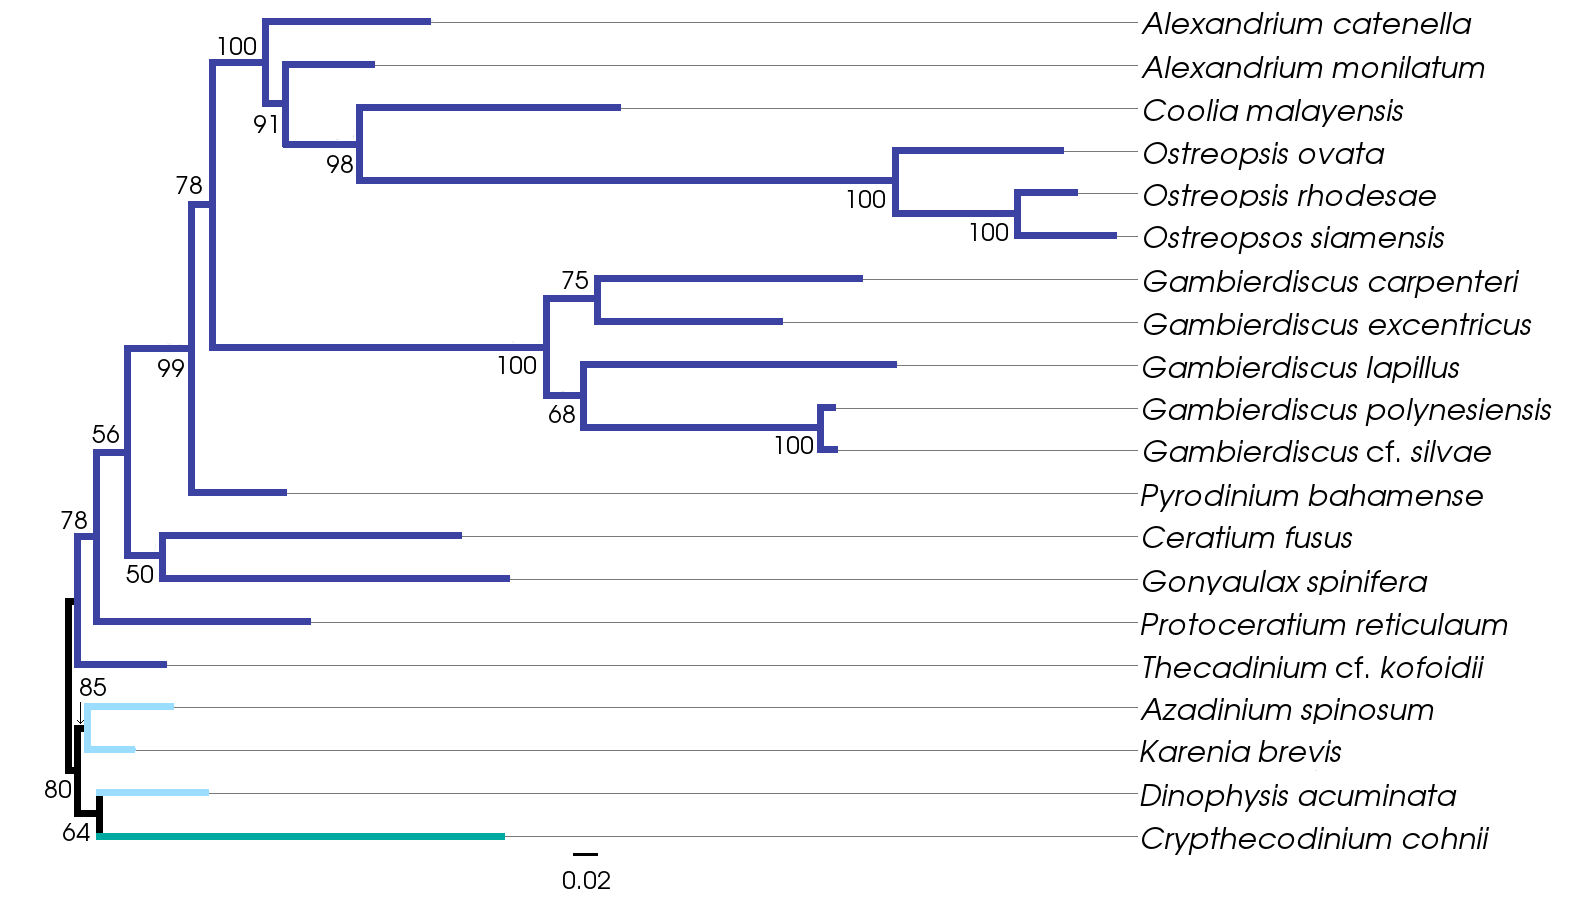
\includegraphics[scale=.4]{figures/rDNA-ML.png} 
\caption{Maximum likelihood phylogenetic inference of ribosomal DNA genes. Concatenation of small subunit rDNA and D1-D3 region large subunit rDNA. Accession numbers for concatenated genes in Table S3. Gonyaulacales (\#16) in purple, outgroups (\#3) in light blue and taxa \textit{incertae sedis} (\#1) in teal. The scale represents number of mutations.} 
\label{fig:rdna}
\end{figure} 
\FloatBarrier

\subsubsection*{Concatenated single copy gene based phylogeny inferred with ML}
\FloatBarrier
All nodes except one within the \emph{Gambierdiscus} species cluster resolved relatively well supported (Fig. ~\ref{fig:SCconcatML}). 
Species of the genera \emph{Alexandrium}, \emph{Gambierdiscus} and \emph{Ostreopsis} cluster as individual clades with their sister species.  
The topology shows three distinct, well supported clades: 
One encompassing \emph{Alexandrium}, \emph{Coolia} and \emph{Ostreopsis}; another which only contains \emph{Gambierdiscus}; and one which includes \emph{Pyrodinium}, \emph{Gonyaulax} and \emph{Protoceratium}. 
Sister to these clades is \emph{Thecadinium}, followed by \emph{Ceratium}. .
The split of the outgroup was fully supported, while the internal nodes resolved very well supported. 
\emph{Crypthecodinium} resolved within the outgroup, sister to \emph{Karenia.} 
Other deeper nodes were well supported.
 
\begin{figure} 
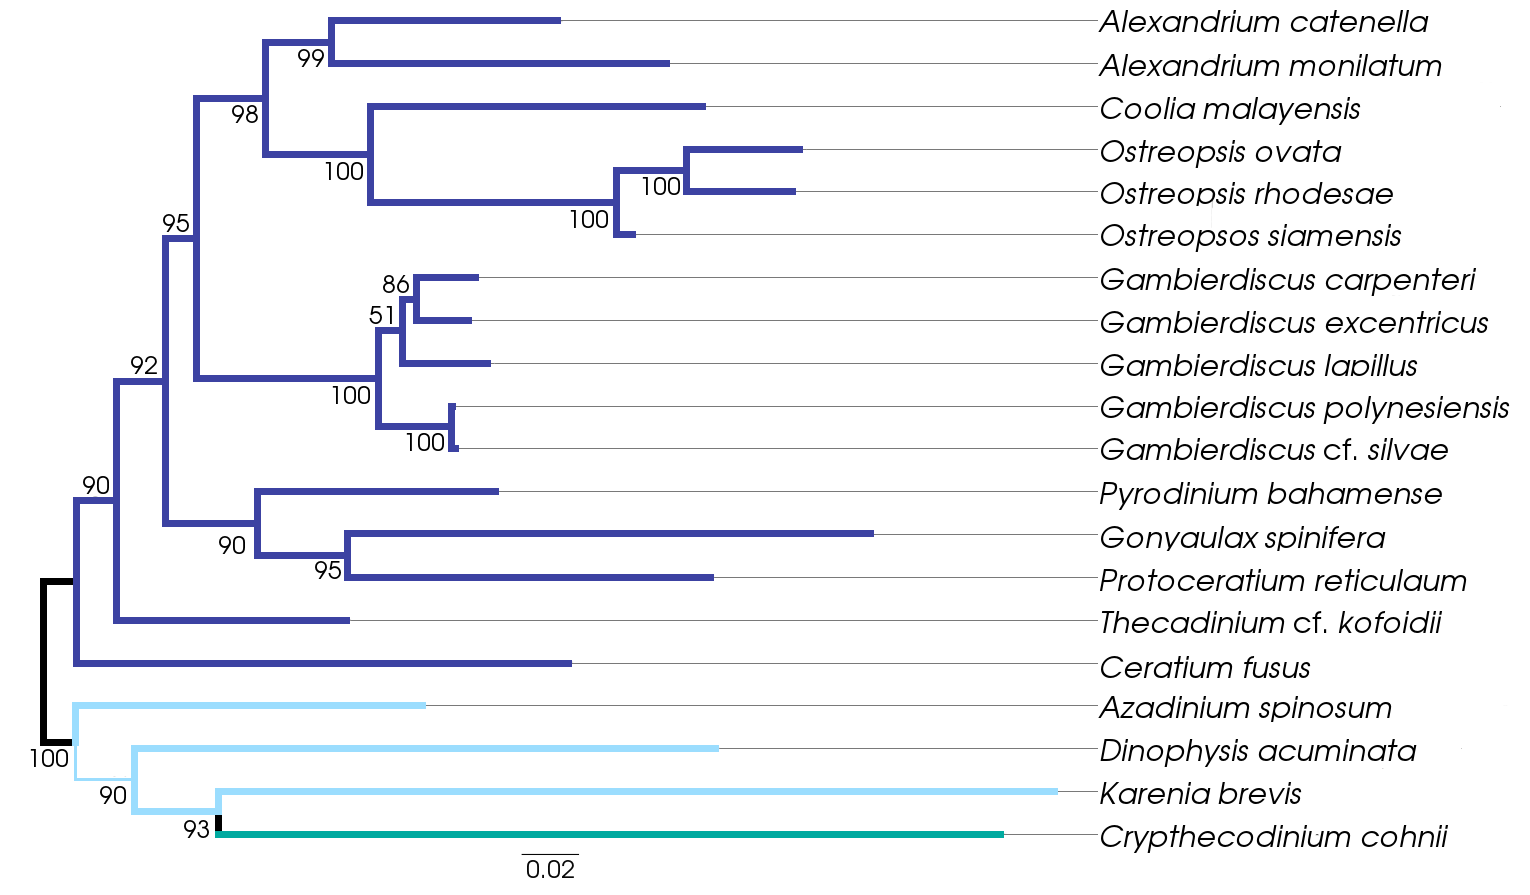
\includegraphics[scale=.45]{figures/Singlecopy-concat-ML.png} 
\caption{Maximum likelihood phylogenetic inference of concatenated single copy gene set (62 single copy genes from 20 taxa). Gonyaulacales (\#16) in purple, outgroups (\#3) in light blue and taxa \textit{incertae sedis} (\#1) in teal. The scale represents number of mutations.} 
\label{fig:SCconcatML}
\end{figure} 
\FloatBarrier

\subsubsection*{Concatenated single copy gene based phylogeny inferred with BI}
\FloatBarrier 
%TODO Running with PATH sampling

\begin{figure} 
%\includegraphics[scale=.23]{} 
\caption{Bayesian inference phylogenetic inference of concatenated single copy gene set (62 single copy genes from 20 taxa). Gonyaulacales (\#16) in purple, outgroups (\#3) in light blue and taxa \textit{incertae sedis} (\#1) in teal.} 
\label{fig:SCconcatBI}
\end{figure} 
\FloatBarrier

\subsubsection*{Single copy gene based phylogeny under MSC}
\FloatBarrier 
All nodes except one within the outgroup clustering resolved (Fig. ~\ref{fig:SCmscBI}). 
Species of \emph{Alexandrium}, \emph{Ostreopsis} and \emph{Gambierdiscus} resolved well or fully supported within their genus clades. 
The topology within the gonyaulacales resolves as three clades: 
one fully suppoerted encompassing \emph{Alexandrium}, \emph{Coolia} and \emph{Ostreopsis}; 
a well supported clade with \emph{Gambierdiscus} and \emph{Pyrodinium}; 
and a supported clade including \emph{Ceratium}, \emph{Gonyaulax}, \emph{Protoceratium} and \emph{Thecadinium}. 
The outgroup clustered together with high support. 
\emph{Crypthecodinium} resolved as a sister taxon to the outgroup. 
Other deeper nodes were well or fully supported.

\begin{figure} 
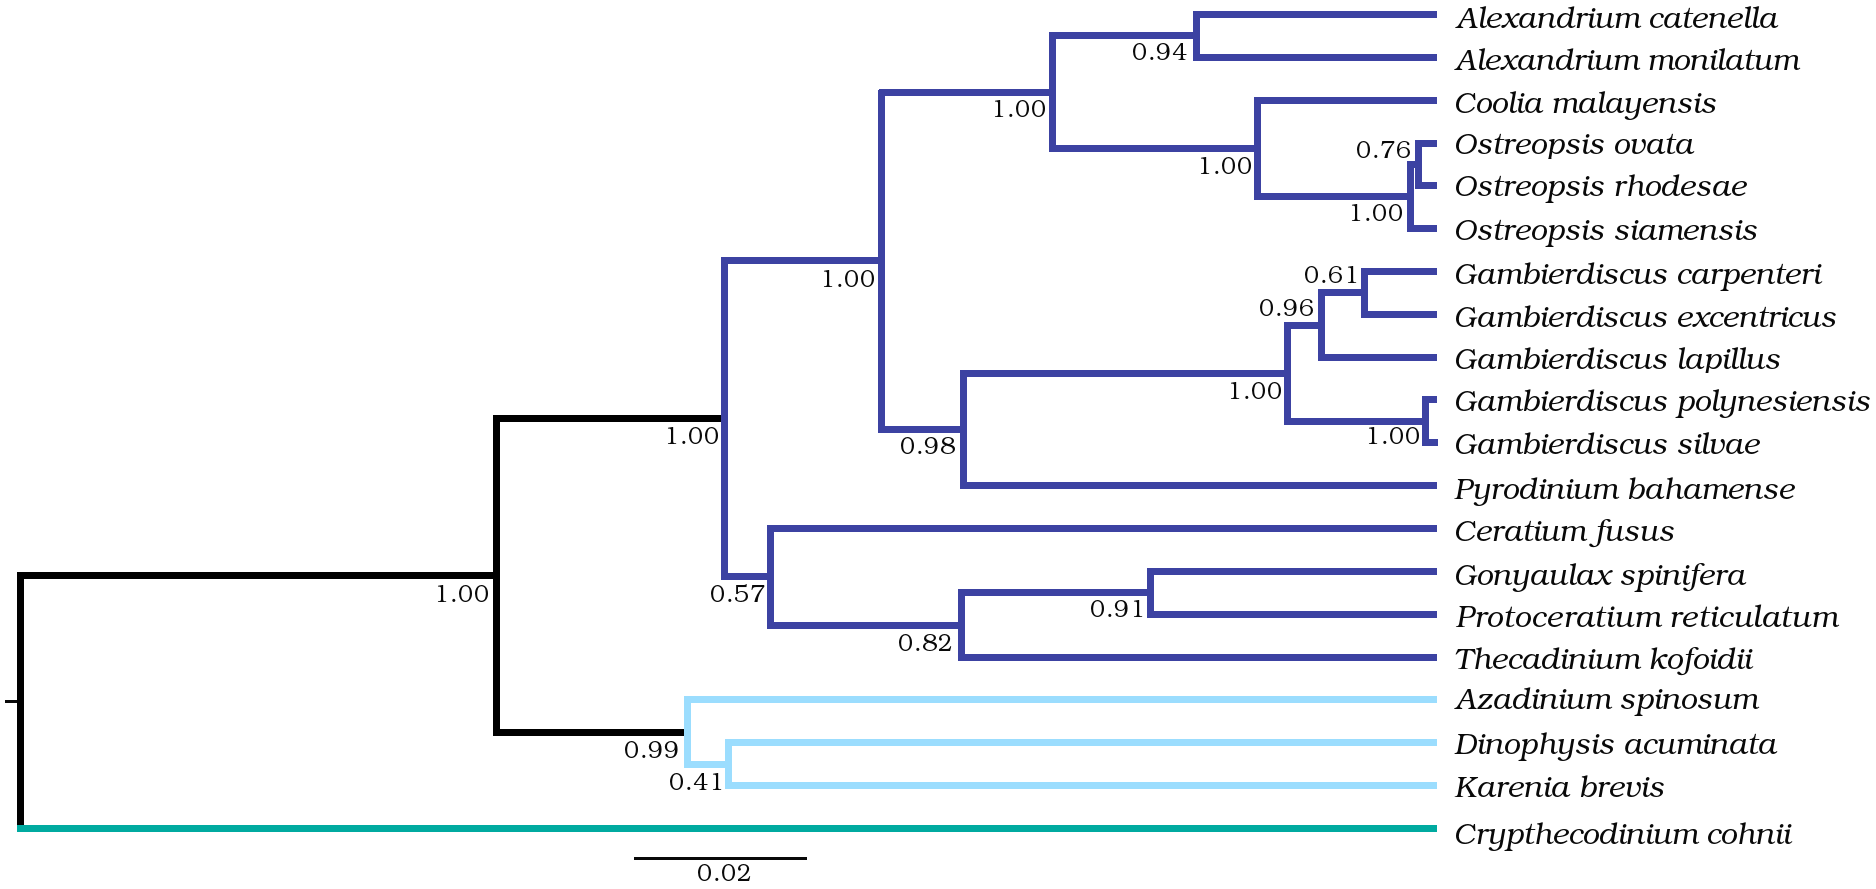
\includegraphics[scale=.25]{figures/Aug2_20-taxa-combined-fig_MCC_trees.png} 
\caption{Phylogenetic analysis of Gonyaulacales species tree with 62 single copy genes from 20 taxa. Gonyaulacales (\#16) in purple, outgroups (\#3) in light blue and taxa \textit{incertae sedis} (\#1) in teal.} 
\label{fig:SCmscBI}
\end{figure} 
\FloatBarrier

\newpage
\section{Discussion}
%TODO work out what UCLN is and re-run rDNA phylo
With publicly available libraries such as the MMETSP project for marine microbes \cite{keeling2014marine}, previous data based limitations for exploring the species evolution within these abundant organisms can be overcome. 
However, the next obstacle lies in the methodology used for investigating the evolutionary relationship between these taxa, as common practice does not necessarily equate best practice.
In particular and highly relevant to working with dinoflagellate phylogenetics, the process of paralog elimination as input for species inference presented here is transparent and, the authors hope, reproducible with basic programming skills. 
Due to the size of their genomes and extensive paralogs the gonyaulacales were chosen to test the methodology presented here.
We present a synopsis of the impact of model and data selection on the overall topology, while comparing commonly employed methodologies. 
The authors are mindful that overparameterization as well as under parameterization can cause mis-specification under BI, if the inference is not in the Felsenstein zone. 
However under- compared to over-parameterization has been shown to have  more severe impacts in giving the wrong species tree \cite{lemmon2004importance}. 
Hence integral to this study was the statistical comparison of different models through PATH sampling as evidence for model parameter adequacy. 
The scripts which form the basis of this study are publicly available through github and the single copy genes used to infer the species evolution in this study, as well as the log files for the *BEAST runs, are available on zenodo. 
What follows is a discussion of the key methodological questions that this study sought to address, using the gonyalacales as a case study. 
%TODO refs:
% LBA usually Parsimony problem, but if the underlying model is mis-specified, occurs in ML & BI
% Disagreements in deeper branches in insect phylogenomic study which compared models - but used concat \cite{boussau2014strepsiptera}
% PATH sampling also penalises over-parameterization \cite{} because while bias decreses w/ #parameters, variance increases. So model \& it's parameters should hit the sweet spot between the two \cite{kelchner2007model}

%Paragraph I reckon I can take out:
%This study presents a set of scripts that trim and assemble RNA-seq libraries, then search for a set of single copy genes common among the input transcriptomes which are subsequently aligned and ready for phylogenetic inference. 
%We demonstrate that this set of methodologies adequately performs despite extensive paralogy in the test organisms, the gonyaulacales.
%sentence on result
%We then demonstrated the impact of data selection on topology by comparing inferences with commonly utilised rDNA sequences and the single copy gene informed phylogeny. 
%sentence on result
%To show the impact of model selection on topology we compared the outcome of applying ML using concatenation vs. BI under coalescence approaches to both datasets. 
%sentence on result
%Finally to assess the better model fit between concatenation and coalescence on the single copy gene dataset, PATH sampling was run. 
%sentence on result
%change depending on PATH sampling
%In relation to the gonyalacales and other similarly difficult taxa, this study presents a data driven, statistically sound method to approach the issue of paralogy for phylogenetics. 
%The approach is founded on identifying single copy genes in transcriptomes; extracting and aligning the candidate genes; and running phylogenetic inference. 
%upt ot here
%The method was tested on taxa  from the order gonyaulacales, class Dinophyceae, with publicly available transcriptomes as well as transcriptomes presented as part of this study. 

%\subsection*{Assessment of methods tested in this study}

%comparison of bootstraps and PP with sim data, they freak out a bit over neither hitting the right answer \cite{erixon2003reliability}
\subsection*{Quality of transcriptome assemblies.}
%Several studies have inferred the evolutionary relationship within the gonyaulacales as part of larger studies around the dinoflagellates, and as such the number of taxa from within the gonyaulacales is too limited to speculate on the families or clades within the order, e.g. \cite{shalchian2006combined,zhang2007three,saldarriaga2004molecular,hoppenrath2010dinoflagellate,murray2005improving}.
Since the publicly available MMETSP datasets, several studies have utilised a broader range of taxa to explore evolutionary stories involving the gonyaulacales. 
However, these have relied on the assemblies supplied as part of the project. 
The stringency of quality trimming of RNA-seq libraries prior to assembly plays a role in the number of unique contigs recovered and the subsequent assembly quality of transcriptomes. 
Regarding the transcriptome assembly method, Cohen et al. evaluated the publicly available assemblies from MMETSP using BUSCO scores, compared to processing and re-assembly with Trinity \cite{cohen-reass}. 
Cohen et al. demonstrated that while the raw data available from the MMETSP project is an excellent resource, the assembly quality is less than ideal. 
Another factor in assembly quality is RNA-seq library processing prior to assembly, especially trimming. 
Commonly high stringency is favored, however MacManes (2014) found that this can be detrimental to the assembly and the quality cut off scores used in this study were based on the recommendation with that study \cite{macmanes2014optimal}.
In short, the trimming and assembly pipeline used for the assemblies available as part of MMETSP have become outdated and this is reflected in the quality comparison by Cohen et al. 
To address this problem, trimming and assembly of RNA-seq libraries using Trimomatic and Trinity respectively were considered integral to the transcriptome assembly in this study.

\subsection*{Quantity of taxa in phylogenetic inference}
%ILS and LBA studies go here - especially Liu 14 \cite{liu2014coalescent}
%TODO so the taxon sampling is important and can reduce bias. nee to work out if enough coverage in the study here, or suggest in limitations \cite{heath2008taxon}
%eukaryotic deep lineages show evidence of rapid diversification \cite{he2016reducing} -- actually maybe find a different ref for this, they're kinda shite, which results in short internl brnaches which is the play ground for ILS.
% \cite{degnan2006discordance} describes that methods which rely on democratic elucidation of species tree by most common gene tree are statistically predisposed to being wrong as anomalous gene trees are likely with asymetric trees, and this holds true for any trees with 5 or more taxa (ie. if there are long and short branches). uses coalescence as example

%\subsection*{Comparison of models tested in this study} 
%As a result we present a phylogeny with good support values, a range of taxa that covers 5 of the 9 families with the gonyaulacales proposed by algaebase, which is the taxonomy authority for phycology journals, e.g. Journal of Phycology. 
%This is likely due to the methodological differences: 
%TODO need to explain these sections in more detail & increase studies compared to, not just gonya
%TODO focus on comparison of own data first
\subsection*{Inferring species evolution from a small subset of genes such as ribosomal genes, whose evolution may not reflect that of the species.}
\FloatBarrier 
% Alveolates rDNA copies some of the highest extreme long branch content \cite{he2016reducing}
% gene tree discordance refers to the common issue of gene tree resolving different to species tree. However historically gene trees were used as an approximation for species tree - which we now know is statistically bollocks \cite{degnan2009gene}. The use of rDNA genes as species estimator is an example of this
Using LSU or SSU rDNA regions for phylogenetics is common practice, at times supplemented with a small number of other genes \cite{shalchian2006combined,zhang2007three,saldarriaga2004molecular,murray2005improving,hoppenrath2010dinoflagellate} 
It is important to acknowledge that these represent the evolutionary history of highly conserved genes, which does not necessarily represent the species evolution. 
Hence studies which utilise primarily rDNA genes for inferring species phylogeny run the risk of presenting the evolutionary history of rDNA genes as synonymous with species evolution when they are in fact poor representatives of the evolutionary history of the majority of nuclear genes?
To address this obstacle, a range of genes need to be used to infer the species evolution.

\begin{figure} 
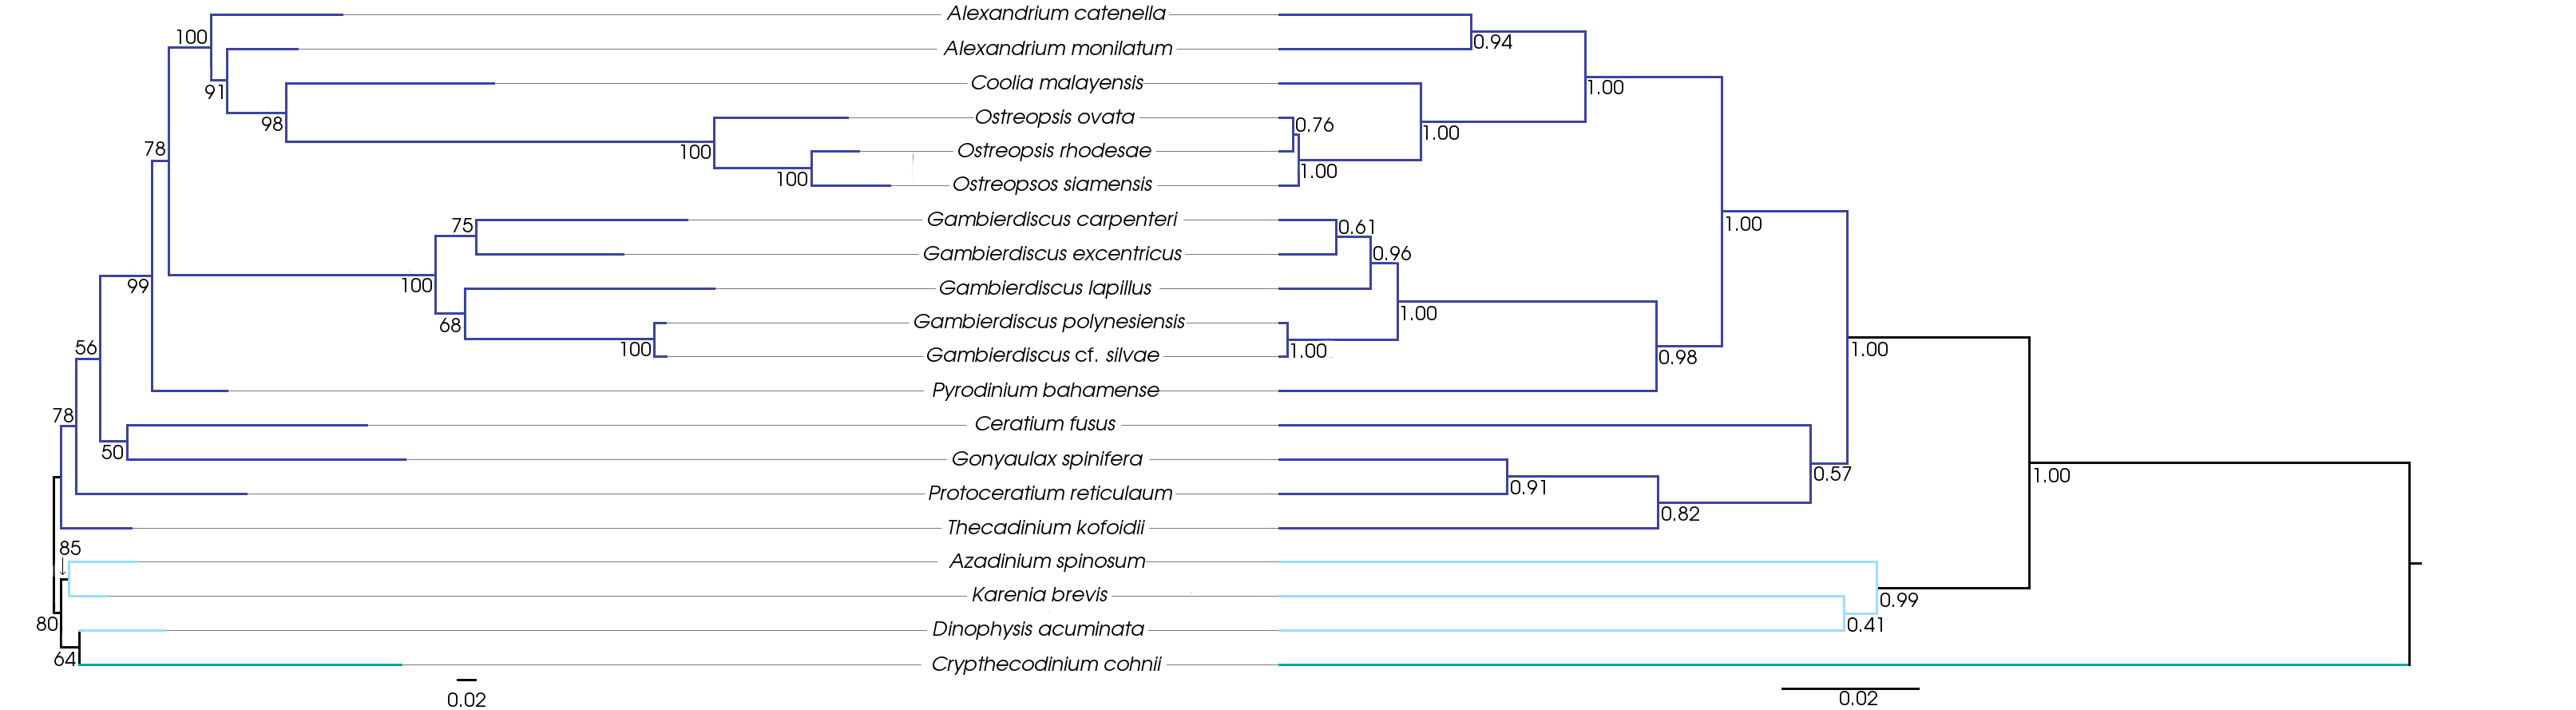
\includegraphics[scale=.2]{figures/MSC-BI_vs_rDNA-ML.png} 
\caption{Tanglegram showing the topological differences in phylogenies from (A) MSC starbeast inference with 58 single copy genes; and (B) concatenated rDNA genes (SSU and D1-D3 LSU)infered with ML. Gonyaulacales (\#16) in purple, outgroups (\#3) in light blue and taxa \textit{incertae sedis} (\#1) in teal.} 
\label{fig:tanglerDNA}
\end{figure} 
\FloatBarrier

\subsection*{Concatenating selected genes and using ML methods for species inference.}
\FloatBarrier
%TODO review on why concatenation is inadequate. assumes uniform evolutionary history across different loci, which is unrealistic. Can cause overinflated confidence through bootstrap values \cite{degnan2009gene}
Concatenation of genes coupled with running ML inference is a commonly used method as it is computationally cheap in comparison to BI methods. 
However as demonstrated by Kubatko et al. (2007) and Roche et al. (2015), this approach is error prone and can be misleading by presenting high bootstrap values on incorrect clades which is positively misleading.
The application of concatenation in combination with ML is common practice in phylogenetic studies for gonyaulacoids  \cite{shalchian2006combined,zhang2007three,saldarriaga2004molecular,murray2005improving,hoppenrath2010dinoflagellate}.
This issue is addressed in this study by running BI under a multi-species coalescence process.
 
\begin{figure} 
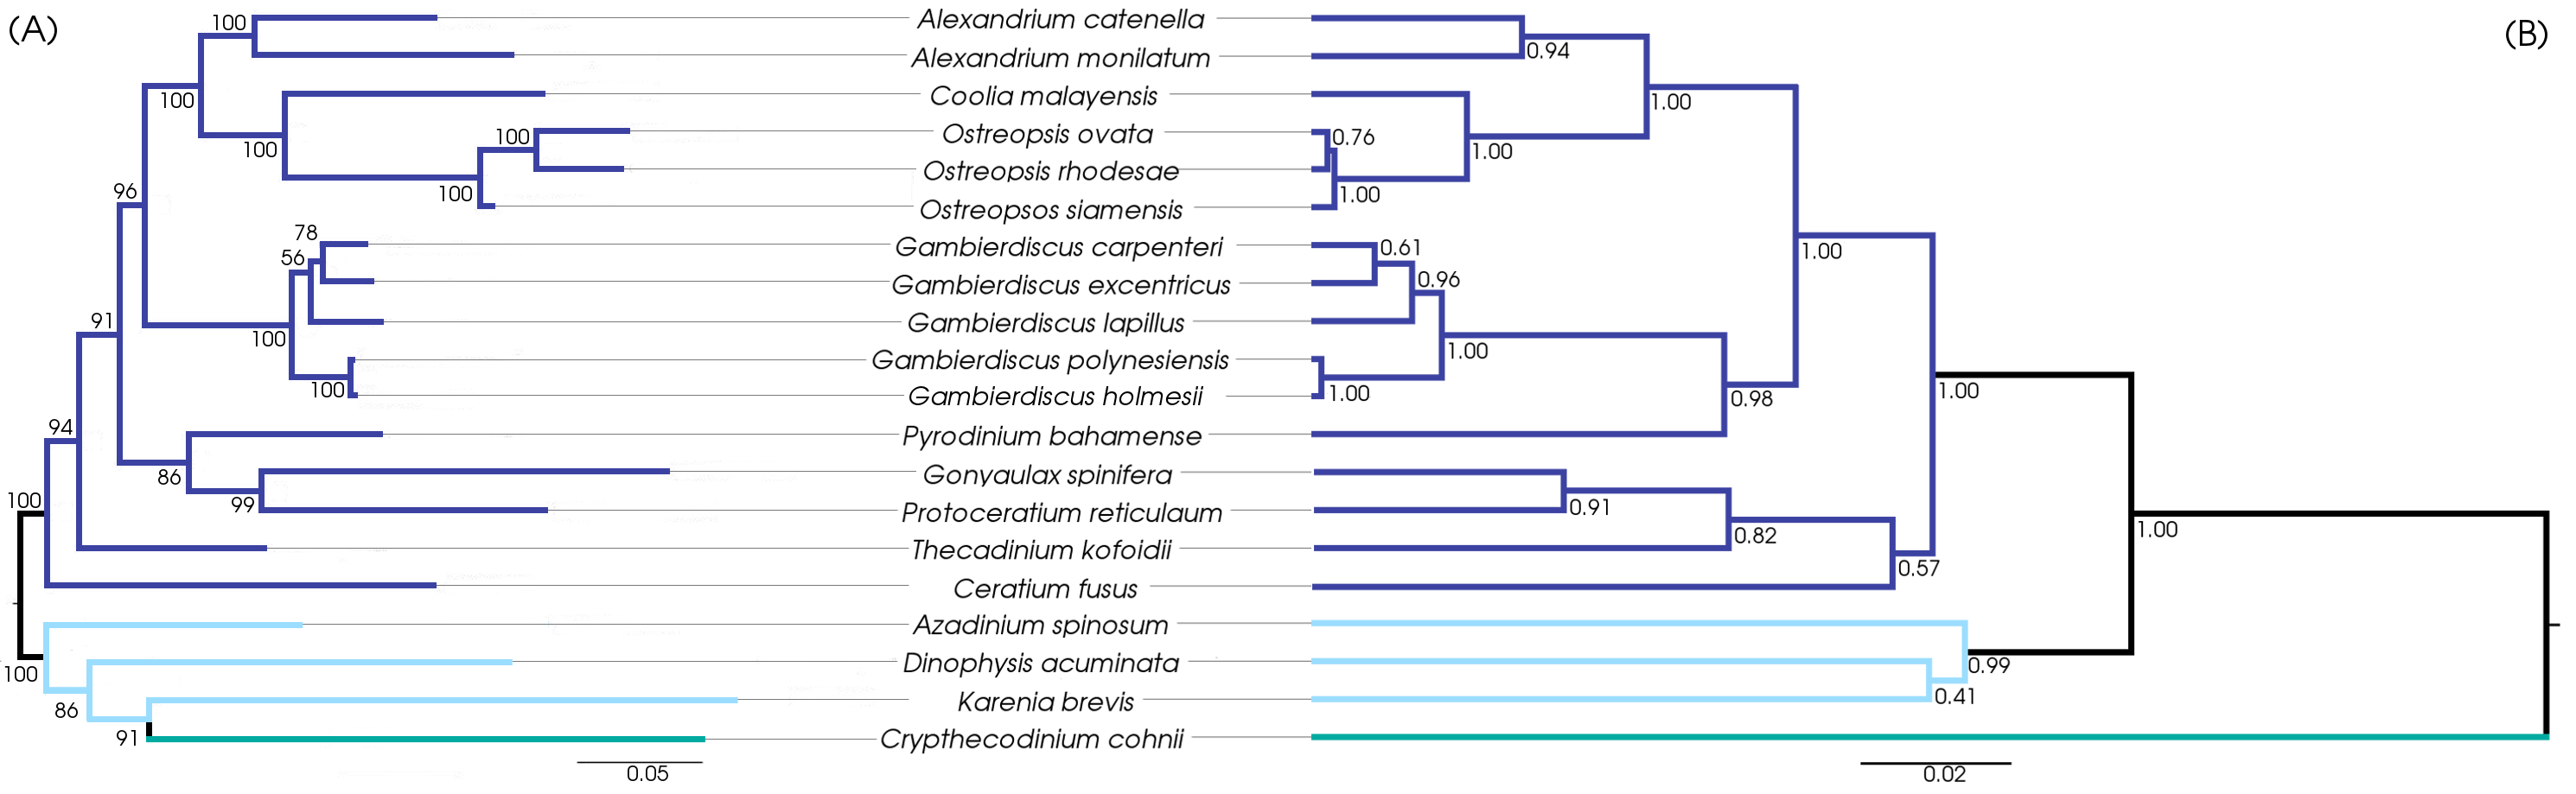
\includegraphics[scale=.2]{figures/MSC-BI_vs_singlecopy-concat-ML.png} 
\caption{Tanglegram showing the topological differences in phylogenies with same 58 single copy gene alignments as input. (A) MSC starbeast inference; and (B) concatenated ML inference. Gonyaulacales (\#16) in purple, outgroups (\#3) in light blue and taxa \textit{incertae sedis} (\#1) in teal.} 
\label{fig:tangleconcatML}
\end{figure} 
\FloatBarrier

\subsection*{Concatenating selected genes and using BI methods for species inference.}
\FloatBarrier 
%with concatenation, coalescent methods still commonly return inaccurate species tree resolutions \cite{kubatko2007inconsistency} 
%Suzuki 2002 shows that PP is overestimated when concatenation is used
%TODO \cite{baele2012accurate} for Path sampling as accurate model assessment method for relaxed clock models... are any improper priors used? PS may not be able to sample from the prior

% MSC robust for both ILS & LBA unlike concat <3 \cite{liu2014coalescent} ; example from water lillies with same phenomenon \cite{liu2014coalescent}

\begin{figure} 
%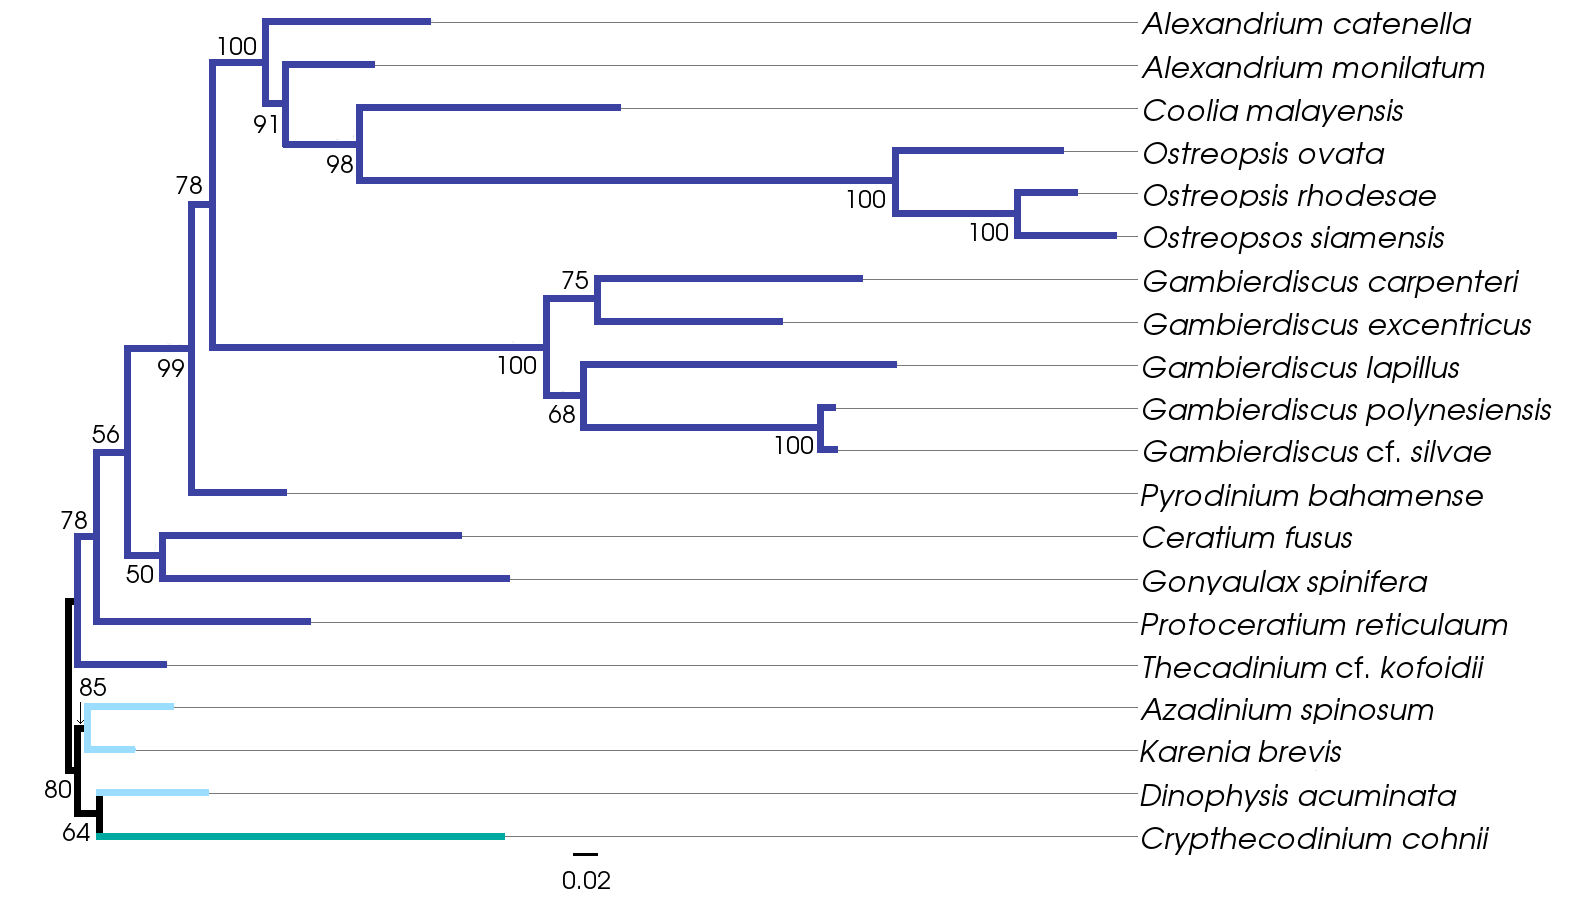
\includegraphics[scale=.23]{figures/rDNA-ML.png} 
\caption{Tanglegram showing the topological differences in phylogenies with same 58 single copy gene alignments as input. (A) MSC starbeast inference; and (B) concatenated beast2 inference. Gonyaulacales (\#16) in purple, outgroups (\#3) in light blue and taxa \textit{incertae sedis} (\#1) in teal.} 
\label{fig:tangleconcatBI}
\end{figure} 
\FloatBarrier

\subsection*{Selection of paralogs to infer species evolution.}
%TODO massively reduce the direct comparison to Price here
%\cite{yang2014orthology} orthologue extr method which means good discussion on problems with wrong selection
%\cite{degnan2009gene} some bullshit bout paralogs in soy bean

Selection of paralogs for species inference is highly problematic as it will compare an arbitrarily divergent gene history as input. 
This problem is particularly prevalent in the dinoflagellates and gonyaulacales due to extensive paralogy from gene duplication. 
Only one other study by Price et al. (2017) seeks to address the issue of parology within the gonyalacales, by purportedly selecting single genes as input. 
However there are several issues with the study presented by Price et al \cite{price2017robust}. 
The assemblies used are from the MMETSP project, which are problematic as mentioned previously as they can present single copy genes which are hybrids of paralogs. 
Hence the selection of single copy genes as input to the species evolution inference, is dubious. 
Further, the methodology for identifying and selecting the single copy genes is not included in the publication. 
Contact with the author established that there was no documentation for the commands that the authors executed, so no record of how the genes were attained was available. 
Hence it was not possible to compare the parameters that went into identifying and screening for single copy genes, it was not possible to scrutinize or reproduce the study.
Lastly, the genes were concatenated and the evolutionary relationships were inferred using ML. While the bootstraps are well supported, this could very well be due to the methodology problems outlined in (2).
The difference in topology between inferences presented by Price et al. and this study, is lies in the organization of sister taxa %(Fig. ~\ref{fig:tangle}). 
Price et al. place \emph{Alexandrium} spp. as the closest genus to \emph{Gambierdiscus}, while this study places \emph{Pyrodinium} as sister. 
As some \emph{Gambierdiscus} spp. produce polyketide toxins which cause ciguatera fish poisoning, establishing the close relations to \emph{Gambierdiscus} is important for investigating the toxin evolution \cite{pawlowiez2014transcriptome}.
The placement of the genus \emph{Azadinium} is equally as divergent as Price et al. place this genus as part of the gonyaulacales, while this study firmly places this genus as an outgroup with \emph{Dinophysis} spp. and \emph{Karenia} spp.
As \emph{Azadinium} spp. also produce polyketide toxins that cause azaspiracid shellfish poisoning, their placement is important for investigating polyketide toxin evolution \cite{meyer2015transcriptomic}.
%\FloatBarrier 
%\begin{figure} 
%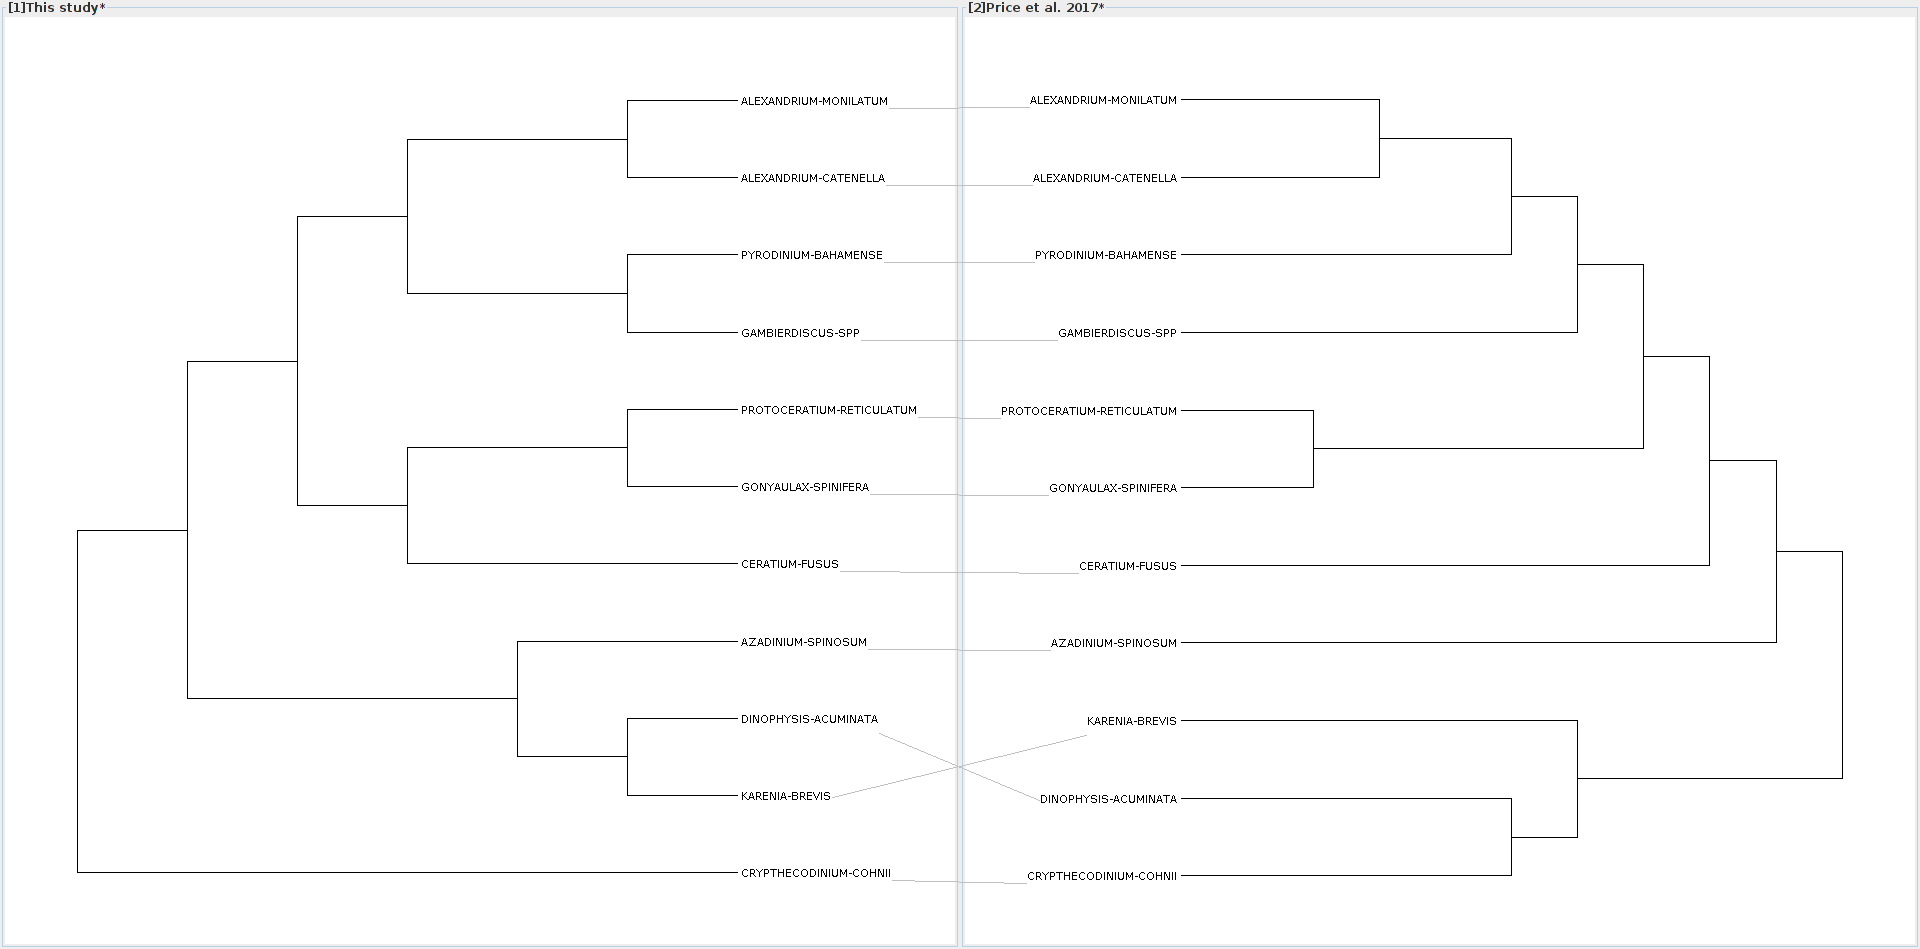
\includegraphics[scale=.23]{Price-comparison.png} 
%\caption{Tanglegram of topology presented in this study (a); and Price et al. (2017) (b). Taxa uncommon to both studies not shown.} 
%\label{fig:tangle}
%\end{figure} 
%\FloatBarrier
In this study, we utilised the BUSCO output which screens for and verifies single copy genes for input into species tree inference, a purpose which was suggested as ideal by the authors of the software \cite{simao2015busco}. 
%AD 160118: you have done a lot of writing describing how previous studies are full of shortcomings and how yours is the awesomest. while that is certainly good for the ego and all, i strongly suggest spending equal effort describing limitations of your study. This gives readers a balanced sense of the work and has the secondary benefit of showing the authors of all those studies you just poopoo'd that you're equally willing to criticize your own work so you are (slightly) less likely to be perceived as an arrogant egomaniac.
% to get you started, perhaps you can talk about the unknown quality of the transcriptome assembly in the regions used for phylo inference. or the fact that you have to do assembly at all instead of just sequencing full length transcripts with high accuracy. or that you have to use transcripts because genomes are too expensive

\subsection*{Limitations of study}
%WAG shows some issues with model misspec under BI using WAG which disappeared with CAT BUT this was based on a concatenated dataset soo... fuck it? \cite{lartillot2007suppression}
In the previous section we identified potential problems with common approaches to species inference for the gonyaulacales, and then sought to demonstrate that our methodology is more robust for addressing these problems. However we in no way want to imply that this study is not fraught with potential pitfalls too. We aim to present avenues for improvement for current methods, especially in areas where large datsets are recently unlocked such as in marine protists with the MMETSP project. %Models and methodology build upon previous work and improve with increased collective knowledge, take the progression for nucleotide substitution rates as an example. The JC69 model from 1969 assumes the substitutions rates between all nuceleotides are equal, including between purines and pyrimidines \cite{}. Through a series of increased complexity to model transition \& transversion rates (i.e. the likelihood of nucleotide change from purine to pyrimidine and vice versa) and steady-state distributions (frequency of each nucleotide given infinite time), the HK85 model was proposed in 1985 \cite{}.
%I may have gone on a tangent here. Probably leave that out.
What follows is the identification of issues with the approach presented in this study, which the authors hope that these will be improved upon in the future. 
%\subsubsection*{Pipeline specific issues}
\paragraph*{Trimming of RNA seq libraries.} The cut off values chosen for this study are based on the recommendations of MacMannes (2014) for optimal transcript discovery. However the recommendations are based on an RNA-seq library from mouse embryonic stem cells, which may not be an adequate model for dinoflagellates. 
This could confound the difference between single copy genes and sequencing artifacts.
%\paragraph*{Single copy gene selection bias.} The selection of single copy genes is based on BUSCOv2 hmmer libraries. The pre-screening process by which may have inherent selection bias that is not tranparent to us // Not sure if this one is a problem =/
\paragraph*{Assembly parameters.}
Trinity was chosen as the assembler for this study based on the findings of Honaas et al. (2016), in which Trinity was one of the top performing assemblers for \textit{de novo} transcriptomes as tested with \textit{Arabidopsis thaliana}, a plant with some similar genetic features to dinoflagellates.
Further, Trinity performed well for identifying isoforms of genes and excelled at assembling highly expressed genes \cite{honaas2016selecting}.
Conversely, Cerveau et al. (2016) found that Trinity, CLC Bio and IDBA-Tran assemblies all contain bioinformatic artifacts. 
Using a combination of all three assemblers yielded a final assembly closer to biological reality than any individual assembler, when no reference genome is available \cite{cerveau2016combining}.
As this study uses Trinity exclusively, it is subject to the bioinformatic errors found by Cerveau et al. which could affect downstream analysis.
%\paragraph*{Amino acid substitution model.} WAG model
%\paragraph*{Molecular clock model selection.} Relaxed clock normal
%\subsubsection*{Gonyaulacales specific issues}
\paragraph*{Contamination of other taxa.} 
The 650+ RNA extract submission to MMETSP was from a large number of investigators and low level contamination is inherent in the project \cite{keeling2014marine}. 
As the cultures tested in all the studies contributing to this dataset were not axenic, contamination could be bacterial or eukaryotic in nature and could result in misleading gene phylogenies which were used to infer the species phylogeny.
\paragraph*{No representative genome for comparison.} 
Without a guided genome comparison, it is difficult to extrapolate on the assembly adequacy and whether the genes selected are single copies, or  mis-assemblies of paralogs.
\paragraph*{Different methods for RNA-seq.} 
Three different approaches for RNA-seq library generation were employed for the libraries used in this study, the MMETSP taxa were sequences on HiSeq platform with 50bp inserts; while all other taxa were sequenced on the NextSeq platform with 75bp or 150bp inserts.
\paragraph*{Total evidence.}
%TODO usingbayesian and fossil dating to infer major eukar group splits, also impacts of age estimations based on model used \cite{eme2014age}

\newpage
\section{Conclusion}
With the accessibility of large data sets, the focus needs to fall on the methodology for investigating them. This study presents a robust methodology to process RNA-seq libraries through assembly, single copy gene selection to phylogenetic species inference. As a case study, the gonyaulacales phylogeny was elucidated as taxa within this order are rife with paralogs. The resulting phylogeny shows a well resolved, well supported inference of the gonyaulacales evolution. By presenting a statistically rigurous methodology and demonstrating how this overcomes common problems faced in phylogenetic studies, we hope that the use of reproducible, open-access processing of large data-sets such as the MMETSP database becomes the standard.  
\newpage

\section{Acknowledgments}
The GVL section of this study was conducted inside the National eResearch Collaboration Tools and Resources (NeCTAR) research cloud, an initiative by the National Research Infrastructure for Australia (NCRIS).
Gratitude to the Stanley Watson foundation, the Linnaean Society of New South Wales, and the ABRS National Taxonomy Research Student Travel Bursary for funding A. L. Kretzschmar's attendance at the Molecular Evolution workshop at the Marine biological laboratory, Woods Hole, MA, USA.
Shout out to the Taming the BEAST organizers \& fellow attendees for a most illuminating workshop in February 2017 on BEAST methodology, and to Geneious for subsidizing A. L. Kretzschmar's attendance fee.
Thank you to Dr. Tim Kahlke for running Interproscan for transcriptome analysis.
\section{Supplementary material}
\FloatBarrier
\begin{table}
\caption{Table S1: Culturing conditions for species processed for this study.}
%\label{tbl:strainTable}
\begin{tabular}{ | p{3cm} | p{2.5cm} | p{1.5cm} | p{5.3cm} |}
\hline
\textbf{Species} & \textbf{Strain}& \textbf{Temp} & \textbf{Source location} \\
%\hline
%\textit{Coolia malayensis}&MAB&& \\
\hline
\textit{Gambierdiscus carpenteri}&UTSMER9A&17&Merimbula, AU\\
\hline
\textit{Gambierdiscus lapillus}&HG4&27&Heron Island, AU\\
\hline
\textit{Gambierdiscus polynesiensis}&CG15&27&Rarotonga, COK\\
\hline
\textit{Gambierdiscus} cf. \textit{silvae}&HG5&27&Heron Island, AU\\
\hline
%\textit{Ostreopsis ovata}&HER27&&\\
%\hline
%\textit{Ostreopsis rhodesae}&HER26&&\\
%\hline
%\textit{Ostreopsis siamensis}&BH1&&\\
%\hline
\textit{Thecadinium} cf. \emph{kofoidii}&THECA&18&Gordons bay, Sydney, AU\\
\hline
\end{tabular}
\end{table}
\FloatBarrier

\begin{longtable}{  | p{3.5cm} |p{2.2cm} | p{1.8cm} | p{1.8cm} | p{1.8cm} | p{3cm} |}
\caption{Table S2: Transcriptomes used for study along including strain ID, source and BUSCOv2 information. MMETSP abbreviation for marine Microbial eukaryotic transcriptome sequencing project, by Moore Foundation.}\\
\hline
%\label{tbl:Transcriptomes}
%\textbf{Family}&
\textbf{Species}&\textbf{Strain}&\textbf{complete BUSCOs}&\textbf{single complete BUSCOs}&\textbf{fragmented BUSCOs}&\textbf{Source}\\
\hline
 \multicolumn{6}{| c |}{Gonyaulacales transcriptomes}\\
    \hline
\emph{Alexandrium catenella}&OF101&110&74&3&MMETSP0790 \citep{keeling2014marine}\\
        \hline
\emph{Alexandrium monilatum}&JR08&107&74&3&MMETSP0093 \citep{keeling2014marine}\\
        \hline
\emph{Ceratium fusus}&PA161109&121&81&4&MMETSP1074 \citep{keeling2014marine}\\
        \hline
\emph{Coolia malayensis}&MAB&138&100&1&(Verma 2018, in prep)\\
\hline
\emph{Crypthecodinium cohnii}&Seligo&126&98&0&MMETSP0326\_2 \citep{keeling2014marine}\\
        \hline
\emph{Gambierdiscus carpenteri}&UTSMER9A&101&83&2&This study\\
\hline
\emph{Gambierdiscus excentricus}&VGO790&88&83&4&\cite{kohli2017role}\\
        \hline
\emph{Gambierdiscus lapillus}&HG4&141&98&2&This study\\
        \hline
\emph{Gambierdiscus polynesiensis}&CG15&104&81&3&This study\\
        \hline
\emph{Gambierdiscus} cf. \emph{silvae}&HG5&134&87&2&This study\\
        \hline
\emph{Gonyaulax spinifera}&CCMP409&83&53&2&MMETSP1439 \citep{keeling2014marine}\\
        \hline
\emph{Ostreopsis ovata}&HER27&132&99&2&(Verma 2018, in prep)\\
     \hline
\emph{Ostreopsis rhodesae}&HER26&131&98&1&(Verma 2018, in prep)\\
     \hline
\emph{Ostreopsis siamensis}&BH1&132&98&1&(Verma 2018, in prep)\\
     \hline
\emph{Protoceratium reticulatum}&CCCM535=CCMP1889&108&72&5&MMETSP0228 \citep{keeling2014marine}\\
    \hline
\emph{Pyrodinium bahamense}&pbaha01&119&897&2&MMETSP0796 \citep{keeling2014marine}\\
        \hline
\emph{Thecadinium} cf. \emph{kofoidii}&THECA&93&70&5&This study\\
 \hline
 \multicolumn{6}{| c |}{Outgroup transcriptomes}\\
 \hline
 \emph{Azadinium spinosum}&3D9&1.8&81&4&MMETSP1036\_2 \citep{keeling2014marine}\\
        \hline
\emph{Dinophysis acimunata}&DAEP01&117&74&2&MMETSP0797 \citep{keeling2014marine}\\
        \hline
\emph{Karenia brevis}&CCMP2229&115&85&2&MMETSP0030 \citep{keeling2014marine}\\
    \hline
\end{longtable}
\FloatBarrier
%families, sections which was taken out:Ceratiaceae,Crypthecodiniaceae,Gonyaulacaceae,Protoceratiaceae,Dinophysiaceae,Dinophyceae incertae sedis,Gymnodiniales

\begin{longtable}{  | p{3cm} |p{3cm} |  p{3cm} | }
\caption{Table S3: Accession numbers for ribosomal DNA sequences used for Fig. ~\ref{fig:rdna}. Sequences sourced from NCBI, except accesion numbers with '$\ast$' sourced from the Silva database. Genes not publically available are denoted by '-'.}\\
\hline
%\label{tbl:Transcriptomes}
%\textbf{Family}&
\textbf{Species}&\textbf{SSU seq.}&\textbf{D1-D3 LSU seq.}\\

\hline
 \multicolumn{3}{| c |}{Gonyaulacales taxa}\\
 \hline
\emph{Alexandrium catenella}&AB088286&AB088238\\
        \hline
\emph{Alexandrium monilatum}&AY883005&-\\
        \hline
\emph{Ceratium fusus}&AF022153&AF260390\\
        \hline
\emph{Coolia malayensis}&HQ897279$\ast$&KX589143\\
\hline
\emph{Crypthecodinium cohnii}&M64245&-\\
        \hline
\emph{Gambierdiscus carpenteri}&EF202908&EF202938\\
\hline
\emph{Gambierdiscus excentricus}&GETL01000157$\ast$&HQ877874\\
        \hline
\emph{Gambierdiscus lapillus}&KU558930&-\\
        \hline
\emph{Gambierdiscus polynesiensis}&EF202907&This study\\
        \hline
\emph{Gambierdiscus} cf. \emph{silvae}&This study&this study\\
        \hline
\emph{Gonyaulax spinifera}&AF022155&DQ151558\\
        \hline
\emph{Ostreopsis ovata}&AF244939&KJ781420\\
     \hline
\emph{Ostreopsis rhodesae}&KX055855&KX055845\\
     \hline
\emph{Ostreopsis siamensis}&KX055868&HQ414223\\
     \hline
\emph{Protoceratium reticulatum}&AF274273&EF613362\\
    \hline
\emph{Pyrodinium bahamense}&AY456115&AB936757\\
        \hline
\emph{Thecadinium} cf. \emph{kofoidii}&AY238478&KT371445\\
 \hline
\multicolumn{3}{| c |}{Outgroup taxa}\\
    \hline
  \emph{Azadinium spinosum}&JN680857&JN165101\\
        \hline
\emph{Dinophysis acimunata}&AJ506972&EF613351\\
        \hline
\emph{Karenia brevis}&EF492504&AY355458\\
\hline
\end{longtable}
\FloatBarrier

\newpage
\bibliographystyle{acm}
\bibliography{gonya.bib}


\end{document}\documentclass[12pt]{article}
 \usepackage[hcentering,bindingoffset=20mm]{geometry}
 \usepackage{placeins}
 \usepackage[numbib]{tocbibind}
 \usepackage{rotating}
\usepackage[square,sort,comma,numbers]{natbib}
 \usepackage{graphicx}
 \usepackage{tabularx}
 \linespread{1.3}
 \usepackage{gensymb}
\usepackage{longtable}
 \usepackage{lscape}
 \usepackage{url}
 \addtolength{\textwidth}{2cm}
 \addtolength{\hoffset}{-1cm}
 
 
 \addtolength{\textheight}{2cm}
 \addtolength{\voffset}{-1cm}
 \setlength{\parindent}{0pt}
 
\title{Trial by phylogenetics - how model and data selection impacts the elucidation of the gonyaulacales (Dinophyceae). $^{1}$}
\author{Key words: Bayesian inference, model selection, gonyaulacales, phylogenetics, transcriptomics}
\date{}

\begin{document}
\maketitle
\paragraph{}Anna Liza Kretzschmar$^{2}$\\
Climate Change Cluster (C3), University of Technology Sydney, Ultimo, 2007 NSW, Australia, anna.kretzschmar@uts.edu.au
\paragraph{}Aaron E. Darling \\
The ithree institute, University of Technology Sydney, Ultimo, 2007 NSW, Australia
\paragraph{}Mathieu Fourment \\
The ithree institute, University of Technology Sydney, Ultimo, 2007 NSW, Australia
\paragraph{}Arjun Verma\\
Climate Change Cluster (C3), University of Technology Sydney, Ultimo, 2007 NSW, Australia
\paragraph{}Shauna Murray\\ 
Climate Change Cluster (C3), University of Technology Sydney, Ultimo, 2007 NSW, Australia
\newpage
\section{Abstract}
\newpage

\section{Introduction}
%
%TODO new direction of paper - model and data impact on phylogenetics. need to re-write intro

%good refs re systematics
%\cite{posada2016phylogenomics} start of special issue discussing systematics. Overview of problems and gold mine of references

%rdna
%\cite{ochieng2007nuclear}  don't even know if this is any good but has rdna of eucalypts

%bullshit refs
%Galtier 08 Dealing with incongruence in phylogenomic analyses : argues against validity of ILS and for natural seletion but using morphology for being the reason why they 'can't be extensive problem in reality'. bacteria only though, doesn't hold this up for vertebrates etc.

%for later:
% fern transcriptome database, rife w paralogy www.onekp.com Rothfels '13 Transcriptome-Mining for Single-Copy Nuclear Markers in Ferns .. but use ML
For most of the history of the field of phylogenetics, the limiting factor was availability of data to infer evolutionary relationships.
Now, the breadth of publicly available in genetic information through next-gen sequencing techniques has allowed for an increasingly complex investigation into the evolutionary relationships between organisms. 
The quest for untangling these relationships is an ongoing process that can help inform a broad range of fields, including epidemiology, toxicology and trophic interactions \cite{mctavish2017and}. %TODO need more refs
The limiting factor now becomes possible errors in the methodology and understanding of the model selection underlying the phylogenetic inference by the operator.
%Advances in sequencing capabilities, computational resources and xxx have seen the use of increasing gene sets and complexity in model selection to inform phylogenetic inference. 
%The decrease in next-gen sequencing technology cost has helped make seq more common - which means that public databases of non-model organism genomes or transcriptomes are getting more betterer (fuck me I word good).
%\cite{yang2014orthology} orthologue extr method which means good discussion on problems with wrong selection
%\cite{degnan2009gene} some bullshit bout paralogs in soy bean
%Phylogenetics assessing large gene sets is becoming common practice.
%The availability of large datasets and breadth of information contained therein is phenomenal. 
%Predominantly the focus is on model organisms, however there has been a concerted effort to push non-model organisms to catch up recently. 
An example is the MMETSP project, sequencing the transcriptomes of over 650 marine eukaryotic microbes \cite{keeling2014marine}. 
This project has unlocked an unprecedented wealth of information to investigate the phylogenetics of some rather prolific branches of the tree of life. 
Here we seek to bridge some of the gap between the theoretical in computational biology and the environmental biologists exploring these types of datasets.
%However, wealth of data alone isn't sufficient for an adequate approximation of the evolution of these organisms - robust methodology is key. 
For phylogenetic inference, the gene representative for each taxa is compared with all other representatives, with the assumption of a shared evolutionary history, i.e. orthology, from which the species evolution is inferred \cite{maddison1997gene}. 
%TODO I think I jumped the gun here a little with the next sentence - explain why there can be an error
Increasing the number of genes used for inferring the species evolution can address any random sampling error, however systematic error(s) can be exacerbated by dataset increase. 
To confound this error, it can return robust support values for the incorrect phylogenetic tree inferred and obfuscate the error inherent in the analysis (see Box 1) \cite{jeffroy2006phylogenomics,roch2015likelihood,kubatko2007inconsistency}. 
Frequent issues for species tree inference arise from:\\
1) Selection of paralogs. If genes with different evolutionary histories are selected, the gene tree will not reflect the history of either paralog and be nonsensical for species tree inference; \\
2) Concatenation of genes. Can be statistically inconsistent estimator of the species tree due to incomplete lineage sorting and concatenation acting as imperfect estimator of species tree topology \cite{roch2015likelihood}; and \\
3) Inference of model adequacy from bootstrap values. Kubatko et al. (2007) demonstrated high bootstrap support under maximum likelihood (ML) inference for incorrect species trees with concatenated gene sets as input \cite{kubatko2007inconsistency}. 
As high bootstrap values are often used as an indicator for robust species topology resolution, this fallacy is particularly problematic if the reader/operator is unfamiliar with the statistical phenomenon (see box 1 for).\\
In this study we aim to build a bioinformatic pipeline that attempts to addresses the issues of paralogy when processing transcriptomic data from non-model organisms, utilises alternative methods to both concatenation and ML inference and investigate the impact that model selection has on topology. 
Specifically, the pipeline assembles RNA-seq datasets, identifies and extracts single copy genes across input taxa with extensive paralogy, and runs Bayesian inference (BI) phylogenetics. 
Finally, to apply the pipeline to the historically difficult order Gonyaulacales (phylum: Dinoflagellata) which are notorious for the issues that the pipeline seeks to address (see box 2 for further information on the gonaylacales).\\




%TODO need to bridge the gap in knowledge for taxonomists
\subsubsection*{Box 1: Statistical nomenclature \& errors this study seeks to address}
For in depth explanations see \cite{yang2014molecular}.\\
\textbf{Maximum likelihood estimate:} 
estimates parameters of a statistical model with maximises the parameter's likelihood function. 
Does not use priors, which means probability functions not applied to model parameters, but only their estimates. 
Model reparametrization does not affect MLE, in effect a static method.\\
\textbf{Bayesian probability:}
infers posterior probability from expectation based prior probability and data based likelihood function.
BI uses probability distributions to describe uncertainty in parameters.
Model reparametrization via priors changes posterior output, i.e. a dynamic method informed by observation.\\
\textbf{Heterotachy:} 
change in evolutionary rates of sites over time, specific to lineage(s).\\
\textbf{Potential statistical error types:}\\
1. random. Sampling based error which decreases and approaches zero as size of dataset approaches infinity.\\
2. systematic. Arises from incorrect model assumptions or problems with the model itself. 
Error type persists and increases as dataset size approaches infinity. 
If strong, can override true phylogenetic signal.\\
\textbf{Incomplete lineage sorting:} discordance of gene evolutionary history with the species evolutionary history causing the phylogenetic species tree to be misinfered.\\
\textbf{Long branch attraction:} phylogenetic phenomenon where distantly related taxa are inferred as close relatives due to systematic error.

\subsubsection*{Box 2: Who/what are the gonyaulacales?}
%TODO Aaron and Mathieu, as non protistologists is this section adequate in explaining why the gonyaulacales were chosen for this work, or would it help to include some of the commented out text?
The gonyaulacales are an order within the phylum dinoflagellata, which are an ancient lineage on the eukaryotic branch of life \cite{moldowan1998biogeochemical}. 
%They play a role in several important ecological processes, as members are represented in aquatic environments, where the cover a diverse niches such as symbionts, parasites and some taxa can cause harmful algal blooms through proliferation and/or neurotoxin production \cite{murray2016unravelling}.
Dinoflagellates possess large genomes (estimated 3.7 to 220 Gbp) \cite{casabianca2017genome}, with extensive paralogy and repetitive short sequences %TODO cite
While the evolutionary relationship of most orders within the dinoflagellates has been inferred with consistently high support values, one order has often escaped elucidation - the gonyaulacales. 
%Analyses for this order commonly combined concatenation and maximum likelihood approaches, which yielded long branch attraction, low confidence values and inconsistent taxon resolution \cite{}. 
Improving upon the species the evolution of the gonyaulaceles has implications for environmental disease monitoring, as neurotoxin production is prevalent in this order and the direct cause of paralytic shellfish poisioning, ciguatera fish poisoning, e.g. \cite{shalchian2006combined,zhang2007three,saldarriaga2004molecular,hoppenrath2010dinoflagellate,murray2005improving}. 
%Specifically the ciguatoxins produced by some \emph{Gambierdiscus} spp. are of interest as the causative agent of ciguatera fish poisoning, a neglected tropical disease with global implications \cite{globalcig}.%, which is predicted to increase in prevalence as climate change progresses \cite{}.



\newpage
\section{Materials and methods}
\subsection*{Culture conditions}
\FloatBarrier
Cultures were isolated from locations as per Table S1 and clonal cultures established by micropipetting single cells through sterile seawater. 
Clonal cultures were maintained in F/10 medium and maintained at temperatures indicated in Table S1. 
%AD 160117: do you think these are actually clonal? Does the term clonal as used in euk microbiology include commensal bacteria? clonal but not necessarily axenic? // Yep, that's spot on - clonal but not axenic. These critters tend to die faster than a snowball in a bushfire without their bacteria

\subsection*{RNA isolation}
\emph{Gambierdiscus} spp. and \emph{Thecadinium} cf. \emph{kofoidii} were harvested during late exponential growth phase by filtration onto 5 $\mu$m SMWP Millipore membrane filter (Merck, DE) and washed off with sterile seawater. 
Cells were pelleted via centrifugation (make of centrifuge) for 10 minutes at 350 rcf. 
Supernatant was decanted and 2ml of TRI Reagent (Sigma-Aldrich, subsidiary of Merck, DE) was added to the pellet and vortexed till dissolved. 
Samples were split in two and transferred to 1.5ml eppendorf tubes. 
Cellular thecae were ruptured by three rounds of freeze-thaw, with tubes transferred between liquid Nitrogen and 95 $^{\circ}$C. 
RNA was extracted as per protocol for TRI Reagent. 
RNA elute was purified with the RNeasy RNA clean up kit EXACT NAME as per protocol(Qiagen). 
DNA was digested with TurboDNAse (Life technologies, subsidiary of Thermo Fischer scientific, AU). 
RNA was quantified with Nanodrop 2000 (Thermo Scientific, Australia) and frozen at -80 $^{\circ}$C until sequencing.
%TODO insert centrifuge, kit name deets
 
\subsection*{Library preparation and Sequencing}
The quality of samples was assessed via Agilent 2100 Bioanalyzer. 
Paired-end sequencing was performed on NextSeq 500 High Output at the Ramaciotti Centre (UNSW, AU) with 75bp insert size for \emph{G. lapillus} and \emph{G.} cf. \emph{silvae}; and 150bp inserts for \emph{G. carpenterii}, \emph{G. polynesiensis} and \emph{T.} cf. \emph{kofoidii}.

\subsubsection*{Publically available transcriptome libraries}
The \emph{Gambierdiscus excentricus} VGO790 transcriptome was downloaded from NCBI under accession ID SRR3348983 \cite{kohli2017role}. 
\textit{Coolia malayensis}, \textit{Ostreopsis ovata}, \textit{Ostreopsis rhodesae} and \textit{Ostreopsis siamensis} sequencing libraries were supplied by Arjun Verma (Verma 2018, in prep). 
RNA seq libraries for all remaining transcriptomes were generated by, and downloaded from, the Marine Microbial Eukaryote Transcriptome Sequencing Project \citep{keeling2014marine}.

\subsection*{Transcriptome processing scripts}
The pipeline is packaged in the Nextflow language \cite{nextflow} for streamlined transferal between high performance computing clusters. 
The workflow is separated into two parts, and modules within the pipeline are written in bash and Python 2.7 \cite{python}, including the pandas module \cite{pandas}, and can be found on github. 
%AD 160118: do you want to give the two parts more descriptive short names? // Better ^___^ but maybe not on the short front
The pipeline was run on the Genomics Virtual Lab (GVL) \cite{afgan2015genomics}.
\subsubsection*{Scripting part 1: Transformers, assemble!}
Individual RNA sequencing libraries are the input, which are then processed through FastQC \cite{fastqc} for quality metrics, sequences are trimmed with Trimmomatic (LEADING:3 TRAILING:3 SLIDINGWINDOW:4:5 MINLEN:25) \cite{bolger2014trimmomatic} and assembled with Trinity v2.4.0 (default settings for paired end libraries) \cite{haas2013novo}. 
Assemblies were then processed with BUSCO2 with the protist specific library \cite{simao2015busco}.
The RNA libraries with 150bp inserts generated as part of this study were also subjected to Digital Normalization \cite{diginorm} prior to assembly, to pool identical transcripts before assembly.                                                                                                                                                                                                                                                                                                                                                                                                                                                                                                                                                                                                                                                                                                                                                                                                                                                                                                                                                                                                                                                                                                                                                                                                                                                                                                                                           
\subsubsection*{Scripting part 2: Klondike gold rush}
The BUSCO2 output from all transcriptomes in the previous script run is the input for the second round. 
Any genes that were present in at least 75 \% of the transcriptomes were indexed, the corresponding contig extracted from the assemblies, aligned with hmmer3.1b2 \cite{eddy2015hmmer} and unaligned regions trimmed.
If several candidate sequences are processed for the same organism, a warning message in the command interface alerts the user before proceeding. 
The output for this section was used as basis for single copy gene phylogenetic inferences in subsequent sections.

\subsection*{Assembly analysis}
Contigs from assemblies were clustered with cd-hit with the flaps T 10 -M 5000 -G 0 -c 1.00 -aS 1.00 -aL 0.005 \cite{fu2012cd}. 
Protein coding regions were predicted with Transdecoder \cite{haas2016transdecoder}.
Amino acid clusters were clustered again with cd-hit with the flags as previously except -c 0.98.
Protein sequences were analysed with interproscan v5.27 with local lookup server \cite{quevillon2005interproscan}.

\subsection*{Phylogenetic inferences}
\subsection{Concatenation phylogenetic inference of rDNA genes}
Ribosomal DNA sequences for the small subunit region as well as the D1-D3 large subunit region were acquired from NCBI \cite{coordinators2017database} or the SILVA rRNA database project \cite{silvaproj}, accession IDs in Table S3. 
Individual genes were aligned using the MUSCLE algorithm a maximum of 8 iterations \cite{edgar2004muscle}, then were concatenated in Geneious v11.3 \cite{kearse2012geneious}.
ML inference was obtained using RaxML \cite{stamatakis2014raxml} with the GTR and GAMMA flags, with 100 bootstraps.

\subsubsection*{Concatenation phylogenetic inference of single copy genes}
Sequences were concatenated and ML inference run as described in the previous section, with the ILGF, GAMMA and PROT flags flags.
BI was run in BEAST2 with the Gamma site model with 4 Gamma category counts under the WAG amino acid model. 
A local random clock was used  under the Birth Death model %TODO MATHIEU what was the end nuber of chains?
Both ML and BI inferences were run the HPCC. 

\subsubsection*{Multispecies coalescence phylogenetic inference of single copy genes}
The pipeline output was processed on the University of Technology Sydney's High-performance computing cluster (HPCC).
%AD 160118: the P in HPC is for performance - not power, though neither adjective is very appropriate for UTS's cluster :( // true that
Species evolutionary inference was based on BI with the *BEAST2 model in BEAST2 \cite{bouckaert2014beast}. 
%TODO make a sensical something as 'Bayesian probability'
The analysis was performed under the WAG substitution model \cite{whelan2001general} with a Gamma distribution for four rate categories. 
A random local clock was employed \cite{drummond2010bayesian}. 
Posterior distributions of parameters were approximated after 300,000,000 generations of MCMC runs with 4 heated and one cold chain, sampled every 5,000 generations  with a burn in of 15\%. 
The inference was run four times to compare convergence of parameters, then log and tree files were merged. 
Log and tree files are available on Zenodo DOI: 
Inference was accelerated using BEAGLE \cite{ayres2011beagle} on the GPU.

\subsection*{Path sampling}
%TODO Mathieu please put details in

\subsection*{Inference run time comparison}
A subset of 14 taxa was selected for a comparison between CPU and GPU inference run time comparison. 
The transcriptome libraries were fed through the pipeline as described, which was set to extract single copy genes present in all of the taxa. 
The resulting alignments were run on *BEAST either on the CPU or GPU.

\subsubsection*{Generation of figures}
Tanglegrams were generated with Dendroscope v3.5.9 \cite{huson2007dendroscope}; images were edited in GIMP \cite{gimp}.
\newpage
\section{Results}
\subsection*{Transcriptomes overview}
Sequencing of transcriptomes for \emph{Gambierdiscus} spp. and \emph{T.} cf. \emph{kofoidii} generated datasets ranging in size from, 143,155,667 to 233,822,334 reads, resulting in 97,634 to 191,224 assembled contigs (table ~\ref{tbl:asmstats}). 
Approximately XX\% to XX\% predicted to be protein coding sequences. 
%TODO Interpro scan, SRA IDs
\FloatBarrier
\begin{longtable}{  | p{3cm} |p{2cm} | p{2cm} | p{2cm} | p{2cm} | p{2cm} |}
\caption{Summary of transcriptome sequencing and assembly statistics.}\\
\hline
\label{tbl:asmstats}
\emph{Sequences:}&\emph{G. carpenteri}&\emph{G. lapillus}&\emph{G. polynesiensis}&\emph{G.} cf. \emph{silvae}&\emph{T.} cf. \emph{kofoidii}\\
\hline
 \multicolumn{6}{| c |}{Sequencing}\\
 \hline
\textbf{SRA accession}&&&&&\\
\hline
\textbf{Raw sequencing reads}&186,422,744&145,366,966&217,031,342&143,155,667&233,822,334\\
\hline
%\textbf{Size (Gb)}&16.92&&19.51&&21.08\\
%\hline
 \multicolumn{6}{| c |}{Assembly}\\
 \hline
 \textbf{Contigs \#}&105,464&148,972&114,622&191,224&97,634\\
\hline
\textbf{Average length (bp)}&607&1,139&633&953&581\\
%\hline
%\textbf{Minimum length (bp)}&201&201&201&201&201\\
\hline
\textbf{Maximum length (bp)}&7,448&12,370&6,608&8,198&7,922\\
\hline
  \multicolumn{6}{| c |}{Transcript clustering \& annotation}\\
\hline
\textbf{\# clusters}&139,699&92,418&139,487&107,766&116,468\\
\hline
\textbf{with protein functional domains}&&&&&\\
\hline
%\textbf{with full annotations}&&&&&\\
%\hline
%\textbf{with Enzyme Codes}&&&&&\\
%\hline
%\textbf{mapped to KEGG pathways}&&&&&\\
%\hline
\end{longtable}

\subsection*{BUSCO output}
Assemblies for all transcriptome datasets used in this study were searched with BUSCOv2 and single copy genes extracted. 
The single copy genes acquired though the BUSCO hmmer libraries curated for protists are reported in Table S2 out of the total 234 genes searched for, as well as accession numbers and identifiers for each transcriptome. 
Single copy genes for each transcriptome used in this study are available on Zenodo DOI:
%TODO single copy genes need ot go up on Zenodo, then link DOI here

\subsection*{Phylogenetic inferences}
Support for branches was interpreted as follows, for ML and BI, respectively: 100\%/1.0 was considered fully supported, above 90\%/0.9 was very well supported, 80\%/0.8 and above was interpreted as relatively well supported and above 50\%/0.5 was considered supported but below was considered unsupported.
As \emph{Azadinium spinosum}, \emph{Dinophysis acuminata} and \emph{Karenia brevis} are considered the outgroup to this study, the unifying branch for these taxa was used to root the tree in all subsequent analyses.
\subsubsection*{rDNA based phylogeny}
\FloatBarrier 
All nodes were supported, with a range of certainty (Fig. ~\ref{fig:rdna}).
Species with the genera \emph{Gambierdiscus} and \emph{Ostreopsis} resolved with their sister species with full support. 
Within the \emph{Gambierdiscus} clade, nodes are either supported or fully supported. 
The two species of \emph{Alexandrium} resolve as well supported closest relatives, but do not form an individual clade. 
Deeper nodes were supported but with less certainty than the crown taxa. 
Two distinct clades can be observed from the topology: One including \emph{Alexandrium}, \emph{Coolia} and \emph{Ostreopsis}; another with only \emph{Gambierdiscus}. 
Sister to these clades, in descending order, was \emph{Pyrodinium}, \emph{Ceratium} and \emph{Gonaulax}, \emph{Protoceratium} and \emph{Thecadinium}. 
The outgroup was relatively well supported and included \emph{Crypthecodinium}. 
Support for deeper nodes varied from supported to well supported.

\begin{figure} 
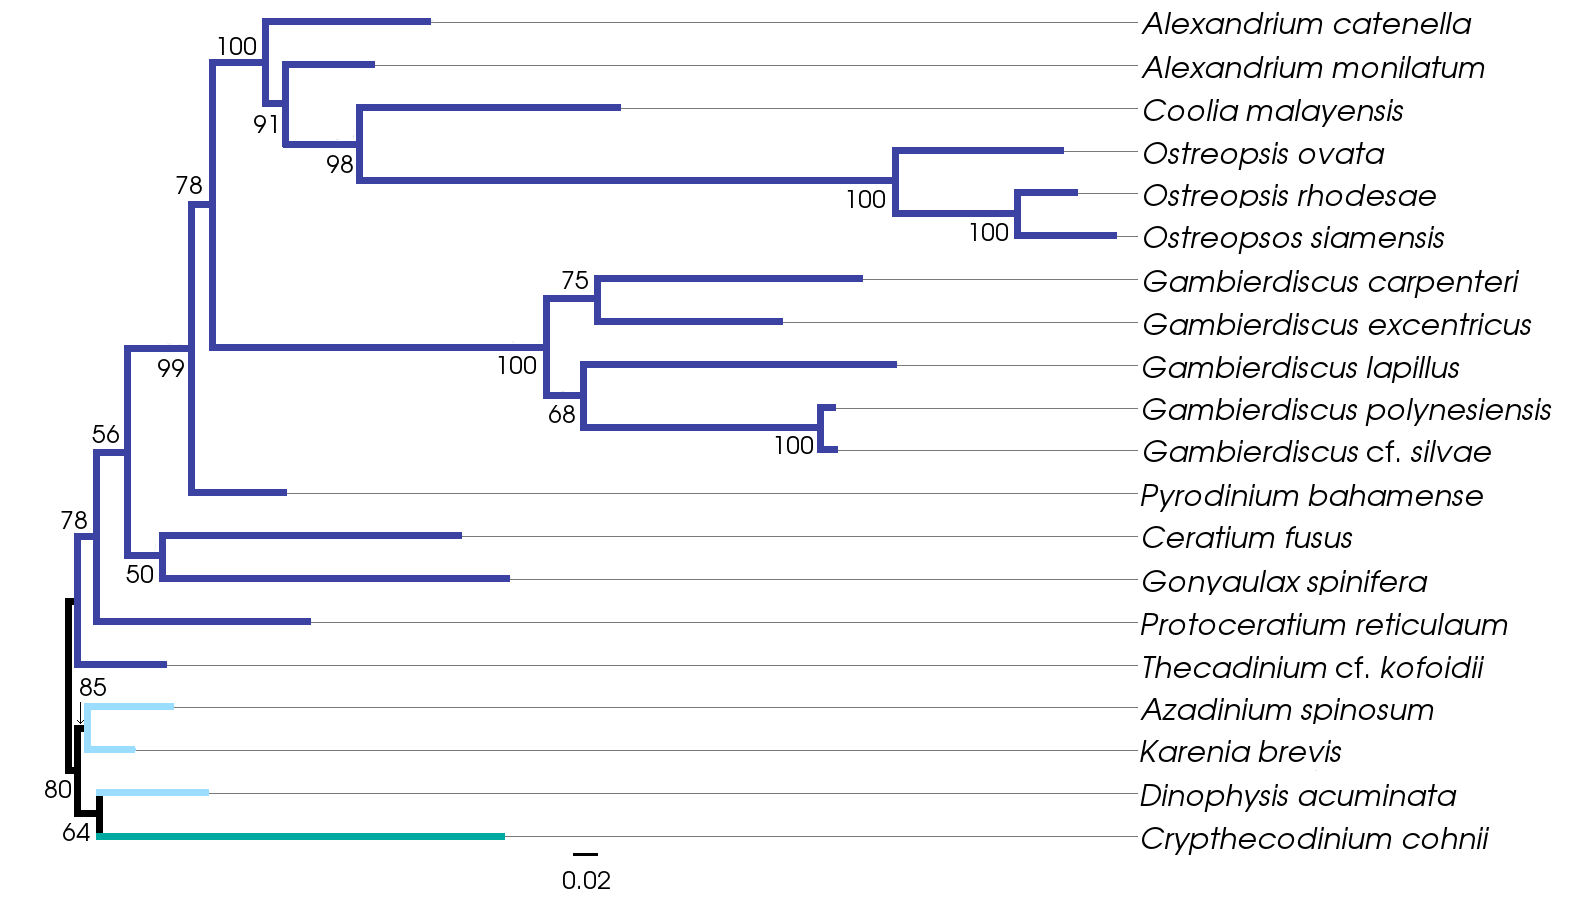
\includegraphics[scale=.4]{figures/rDNA-ML.png} 
\caption{Maximum likelihood phylogenetic inference of ribosomal DNA genes. 
Concatenation of small subunit rDNA and D1-D3 region large subunit rDNA. 
Accession numbers for concatenated genes in Table S3. Gonyaulacales (\#16) in purple, outgroups (\#3) in light blue and taxa \textit{incertae sedis} (\#1) in teal. 
The scale represents number of mutations.} 
\label{fig:rdna}
\end{figure} 
\FloatBarrier

\subsubsection*{Concatenated single copy gene based phylogeny inferred with ML}
\FloatBarrier
All nodes except one within the \emph{Gambierdiscus} species cluster resolved relatively well supported (Fig. ~\ref{fig:SCconcatML}). 
Species of the genera \emph{Alexandrium}, \emph{Gambierdiscus} and \emph{Ostreopsis} cluster as individual clades with their sister species.  
The topology shows three distinct, well supported clades: 
One encompassing \emph{Alexandrium}, \emph{Coolia} and \emph{Ostreopsis}; another which only contains \emph{Gambierdiscus}; and one which includes \emph{Pyrodinium}, \emph{Gonyaulax} and \emph{Protoceratium}. 
Sister to these clades is \emph{Thecadinium}, followed by \emph{Ceratium}. 
The split of the outgroup was fully supported, while the internal nodes resolved very well supported. 
\emph{Crypthecodinium} resolved within the outgroup, sister to \emph{Karenia.} 
Other deeper nodes were well supported.

 
\begin{figure} 
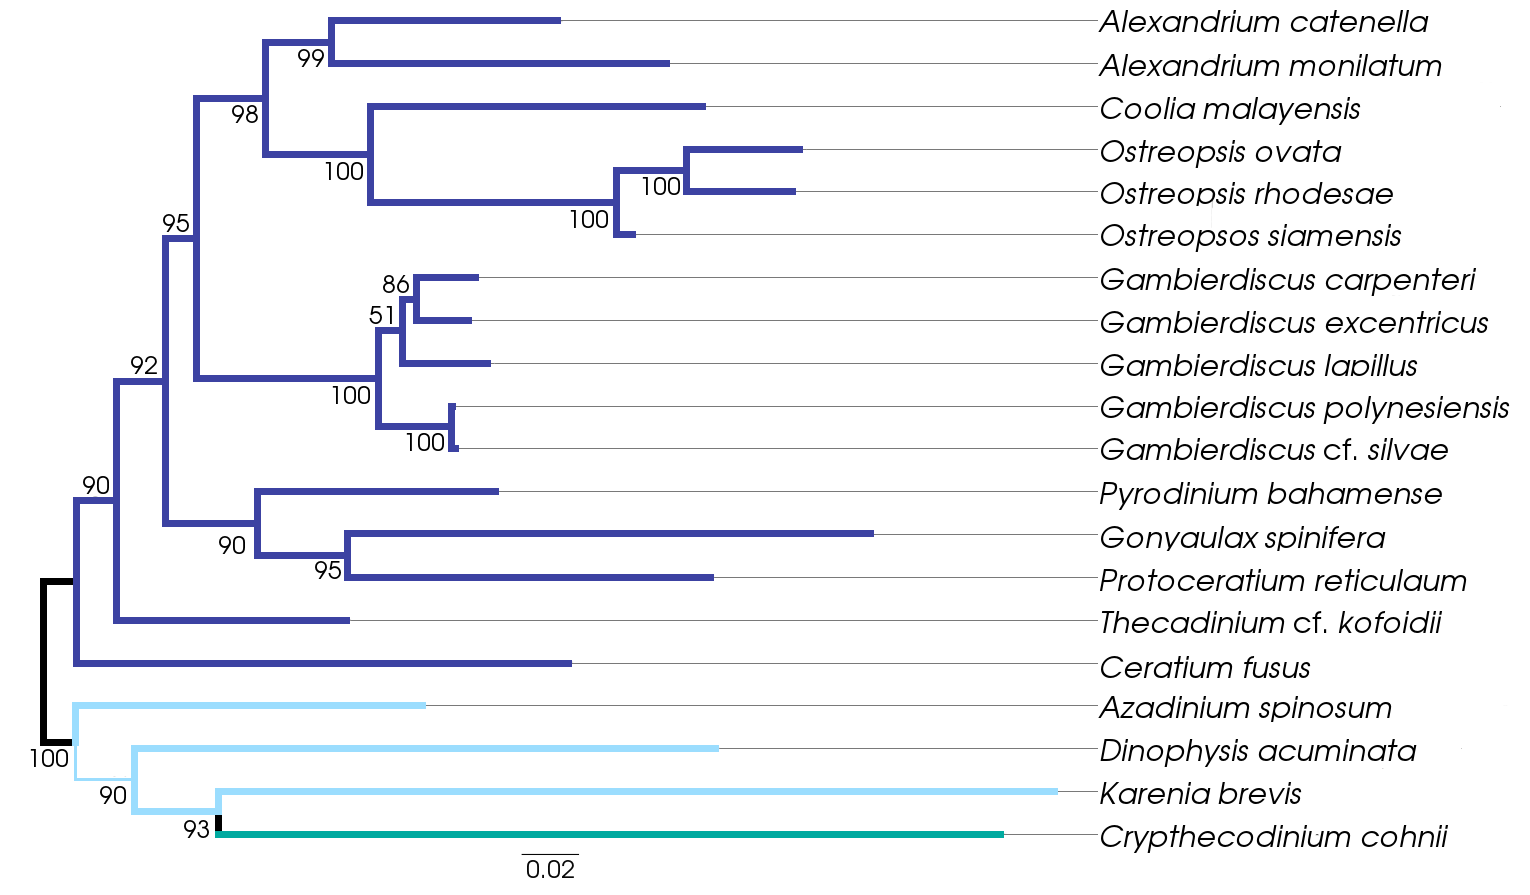
\includegraphics[scale=.45]{figures/Singlecopy-concat-ML.png} 
\caption{Maximum likelihood phylogenetic inference of concatenated single copy gene set (62 single copy genes from 20 taxa). 
Gonyaulacales (\#16) in purple, outgroups (\#3) in light blue and taxa \textit{incertae sedis} (\#1) in teal. 
The scale represents number of mutations.} 
\label{fig:SCconcatML}
\end{figure} 
\FloatBarrier

\subsubsection*{Concatenated single copy gene based phylogeny inferred with BI}
\FloatBarrier 
%TODO Running with PATH sampling

\begin{figure} 
%\includegraphics[scale=.23]{} 
\caption{Bayesian inference phylogenetic inference of concatenated single copy gene set (62 single copy genes from 20 taxa). 
Gonyaulacales (\#16) in purple, outgroups (\#3) in light blue and taxa \textit{incertae sedis} (\#1) in teal.} 
\label{fig:SCconcatBI}
\end{figure} 
\FloatBarrier

\subsubsection*{Single copy gene based phylogeny under MSC}
\FloatBarrier 
All nodes except one within the outgroup clustering resolved (Fig. ~\ref{fig:SCmscBI}). 
Species of \emph{Alexandrium}, \emph{Ostreopsis} and \emph{Gambierdiscus} resolved well or fully supported within their genus clades. 
The topology within the gonyaulacales resolves as three clades: 
one fully suppoerted encompassing \emph{Alexandrium}, \emph{Coolia} and \emph{Ostreopsis}; 
a well supported clade with \emph{Gambierdiscus} and \emph{Pyrodinium}; 
and a supported clade including \emph{Ceratium}, \emph{Gonyaulax}, \emph{Protoceratium} and \emph{Thecadinium}. 
The outgroup clustered together with high support. 
\emph{Crypthecodinium} resolved as a sister taxon to the outgroup. 
Other deeper nodes were well or fully supported.
%The gonyaulacales resolved as a monophyletic order with three major clades, tentatively named clades I - III. 
%Posterior probability (PP) branch support values were analyzed as follows: 1.00 was fully supported, $\geq$ 0.9 was very well supported, $\geq$ 0.8 was relatively well supported and $\leq$ 0.5 was unsupported.
%The separation of clades I, II and III was fully supported, the PP within the three clades was predominantly fully or very well supported. 
%The exception in clade I was the placement of \emph{OFelsenstein zone. ovata} as sister species to \emph{O. rhodesae} with a PP of 0.76. 
%The exception in clade II was in \emph{G. carpenteri} placement as sister species to \emph{G. excentricus} with a PP of 0.61. In clade III, the placement of \emph{P. bahamense} as basal to the other taxa within that clade was supported with 0.57, while the split off for \emph{T.} cf. \emph{kofoidii} was relatively well supported.
%Other deeper branches were very well supported.
%Clade I within the gonyaulacales contains \emph{Alexandrium} spp., \emph{Coolia malayensis} and \emph{Ostreopsis} spp. 
%Clade II contains \emph{Gambierdiscus} spp. as well as \emph{Pyrodinium bahamense} as sister genus. 
%Clade III contains \emph{Pyrodinium bahamense}, \emph{Ceratium fusus}, \emph{Gonyaulax spinifera}, \emph{Protoceratium reticulatum} and \emph{Thecadinium kofoidii}. 
%This inference suggests that \emph{O. ovata} and \emph{O. rhodeseae} are sister species with \emph{O. siamensis} diverging earlier. 
%This is contrary to the \emph{Ostreopsis} species evolution in the literature to date, which is based on ribosomal genes \cite{verma2016molecular}. 
%The placement of \emph{Gambierdiscus} species from this study follows the species resolution in the literature to date \cite{kretzschmar2017characterization}. 
%\emph{Crypthecodinium chonii} did not resolve within the gonyaulacales (green branch Fig. ~\ref{fig:phylo}), but clustered as an outgroup, more distant that the other outgroup taxa \emph{Azadinium spinosum}, \emph{Karenia brevis} and \emph{Dinohysis acuminata}.
%TODO look up toxin production along branches?

\begin{figure} 
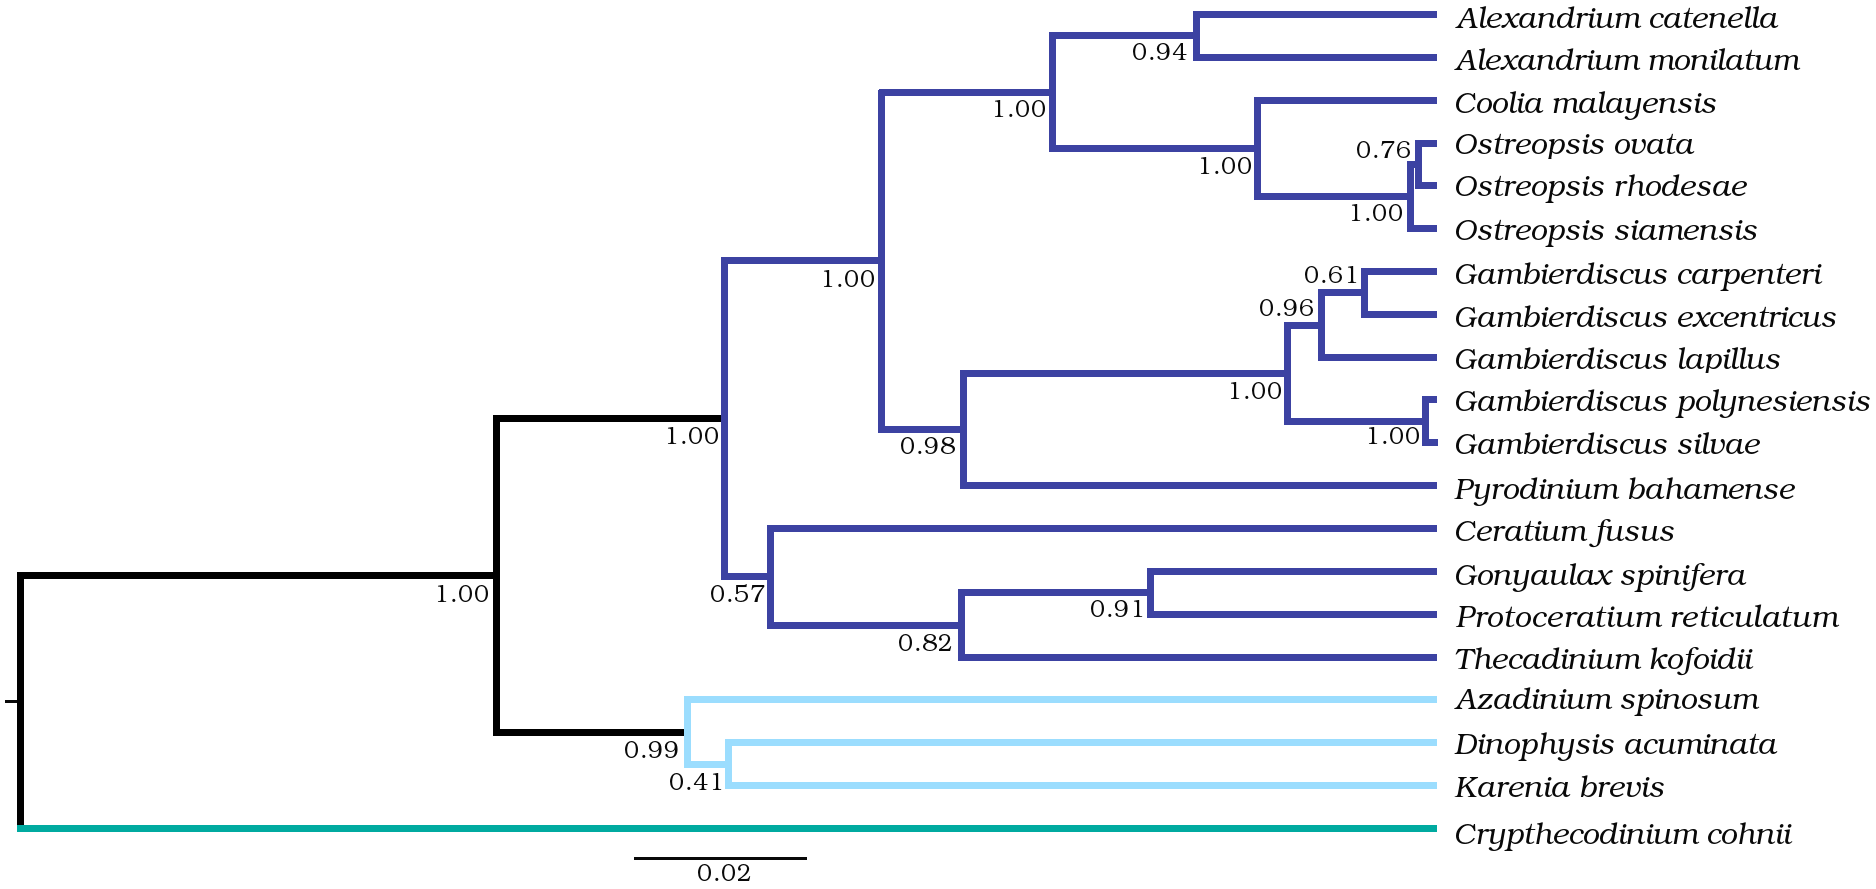
\includegraphics[scale=.25]{figures/Aug2_20-taxa-combined-fig_MCC_trees.png} 
\caption{Phylogenetic analysis of Gonyaulacales species tree with 62 single copy genes from 20 taxa. 
Gonyaulacales (\#16) in purple, outgroups (\#3) in light blue and taxa \textit{incertae sedis} (\#1) in teal.} 
\label{fig:SCmscBI}
\end{figure} 
\FloatBarrier

\newpage
\section{Discussion}

% LBA usually Parsimony problem, but if the underlying model is mis-specified, occurs in ML & BI
This study presents a data driven, statistically sound method to approach the issue of paralogy in datasets for phylogenetics. 
The approach is founded on identifying single copy genes in transcriptomes; extracting and aligning the candidate genes; and running phylogenetic inference. 
The work compares commonly utilized methods of data acquisition and models used to compare the resulting topologies.
The method was tested on taxa from the order gonyaulacales, class Dinophyceae, with publicly available transcriptomes as well as transcriptomes presented as part of this study. 
With publicly available datasets such as the MMETSP project for marine microbes \cite{keeling2014marine}, previous data based limitations for exploring the species evolution within these abundant organisms can now be overcome. 
However, the next obstacle lies in the methodology for investigating these taxa and that is what this study seeks to address. 
The process of paralog elimination as input for species inference presented here is transparent and, the authors hope, reproducible with rudimentary programming skills. 
The gonyaulacales were chosen as a case study to demonstrate the common phylogenetic issues with problematic taxa. 
This scripts for this study are publicly available through github and the single copy genes used to infer the species evolution in this study, as well as the log files for the *BEAST runs, are available on zenodo.

\subsection*{Assessment of methods tested in this study}
Before phylogenetic inference, RNA-seq libraries undergo a number of processing steps which results in assembly and gene selection. 
These steps are integral to the quality of the analysis and can confound efforts before model selection becomes an issue. 
We sought to address these in the following ways: 
\subsubsection*{Quantity of taxa or quality of transcriptome assemblies.}
%ILS and LBA studies go here - especially Liu 14 \cite{liu2014coalescent}
Several studies have inferred the evolutionary relationship within the gonyaulacales as part of larger studies around the dinoflagellates, and as such the number of taxa from within the gonyaulacales is too limited to speculate on the families or clades within the order, e.g. \cite{shalchian2006combined,zhang2007three,saldarriaga2004molecular,hoppenrath2010dinoflagellate,murray2005improving}.
Since the publicly available MMETSP datasets, several studies have utilised a broader range of taxa to explore gonyaulacales evolution. 
However, these have relied on the assemblies supplied by the project. 
The stringency of quality trimming of RNA-seq libraries prior to assembly plays a role in the number of unique contigs recovered and the subsequent assembly quality of transcriptomes. 
Commonly high stringency is favored, however MacManes (2014) found that this can be detrimental to the assembly and the quality cut off scores used in this pipeline were in recommendation with that study \cite{macmanes2014optimal}.
Regarding the transcriptome assembly method, Cohen et al. evaluated the publicly available assemblies from MMETSP, compared to processing and re-assembly with Trinity \cite{cohen-reass}. 
Cohen et al. demonstrated that while the raw data available from the MMETSP project is awesome, the assembly method has become outdated. 
%TODO check veracity of statement: Further, the assembly method used can result in the assembly of paralogs into a single contig, giving the illusion of a single copy gene while actually representing hybrids. 
To address this problem, trimming and assembly of RNA-seq libraries using Trimomatic and Trinity respectively are integral to the pipeline.

\subsubsection*{Selection of paralogs to infer species evolution.}

%\cite{yang2014orthology} orthologue extr method which means good discussion on problems with wrong selection
%\cite{degnan2009gene} some bullshit bout paralogs in soy bean

Selection of paralogs for species inference is highly problematic as it will present an arbitrarily divergent gene history as input. 
This problem is particularly present in the dinoflagellates due to the frequent gene duplication discussed previously (See Box 1). 
Only one other study by Price et al. (2017) seeks to address this by purportedly selecting single genes as input. 
However there are several issues with the study presented by Price et al \cite{price2017robust}. 
The assemblies used are from the MMETSP project which are problematic, as mentioned previously, as they can present single copy genes as are hybrids of paralogs. 
%Hence the selection of single copy genes as input to the species evolution inference, is dubious. 
Further, the methodology for identifying and selecting single copy genes is not included in the publication. 
Contact with the author established that there was no script or documentation for the commands that the authors executed. 
Hence as there is no record of how the genes were attained, it was not possible to examine the parameters that went into identifying and screening for single copy genes, and so it was not possible to scrutinize or reproduce the study for comparison. 
Lastly, the genes were concatenated and the evolutionary relationships were inferred using ML. 
While the bootstraps are well supported, this could very well be due to the methodology problems outlined in the following section. 
In conclusion, the results in this study were not compared to Price et al. (2017) as the methodology for that study was not reproducible or available for statistical comparison. 
%The difference in topology between inferences presented by Price et al. and this study, is lies in the organization of sister taxa %(Fig. ~\ref{fig:tangle}). 
%Price et al. place \emph{Alexandrium} spp. as the closest genus to \emph{Gambierdiscus}, while this study places \emph{Pyrodinium} as sister. 
%As some \emph{Gambierdiscus} spp. produce polyketide toxins which cause ciguatera fish poisoning, establishing the close relations to \emph{Gambierdiscus} is important for investigating the toxin evolution \cite{pawlowiez2014transcriptome}.
%The placement of the genus \emph{Azadinium} is equally as divergent as Price et al. place this genus as part of the gonyaulacales, while this study firmly places this genus as an outgroup with \emph{Dinophysis} spp. and \emph{Karenia} spp.
%As \emph{Azadinium} spp. also produce polyketide toxins that cause azaspiracid shellfish poisoning, their placement is important for investigating polyketide toxin evolution \cite{meyer2015transcriptomic}.
%\FloatBarrier 
%\begin{figure} 
%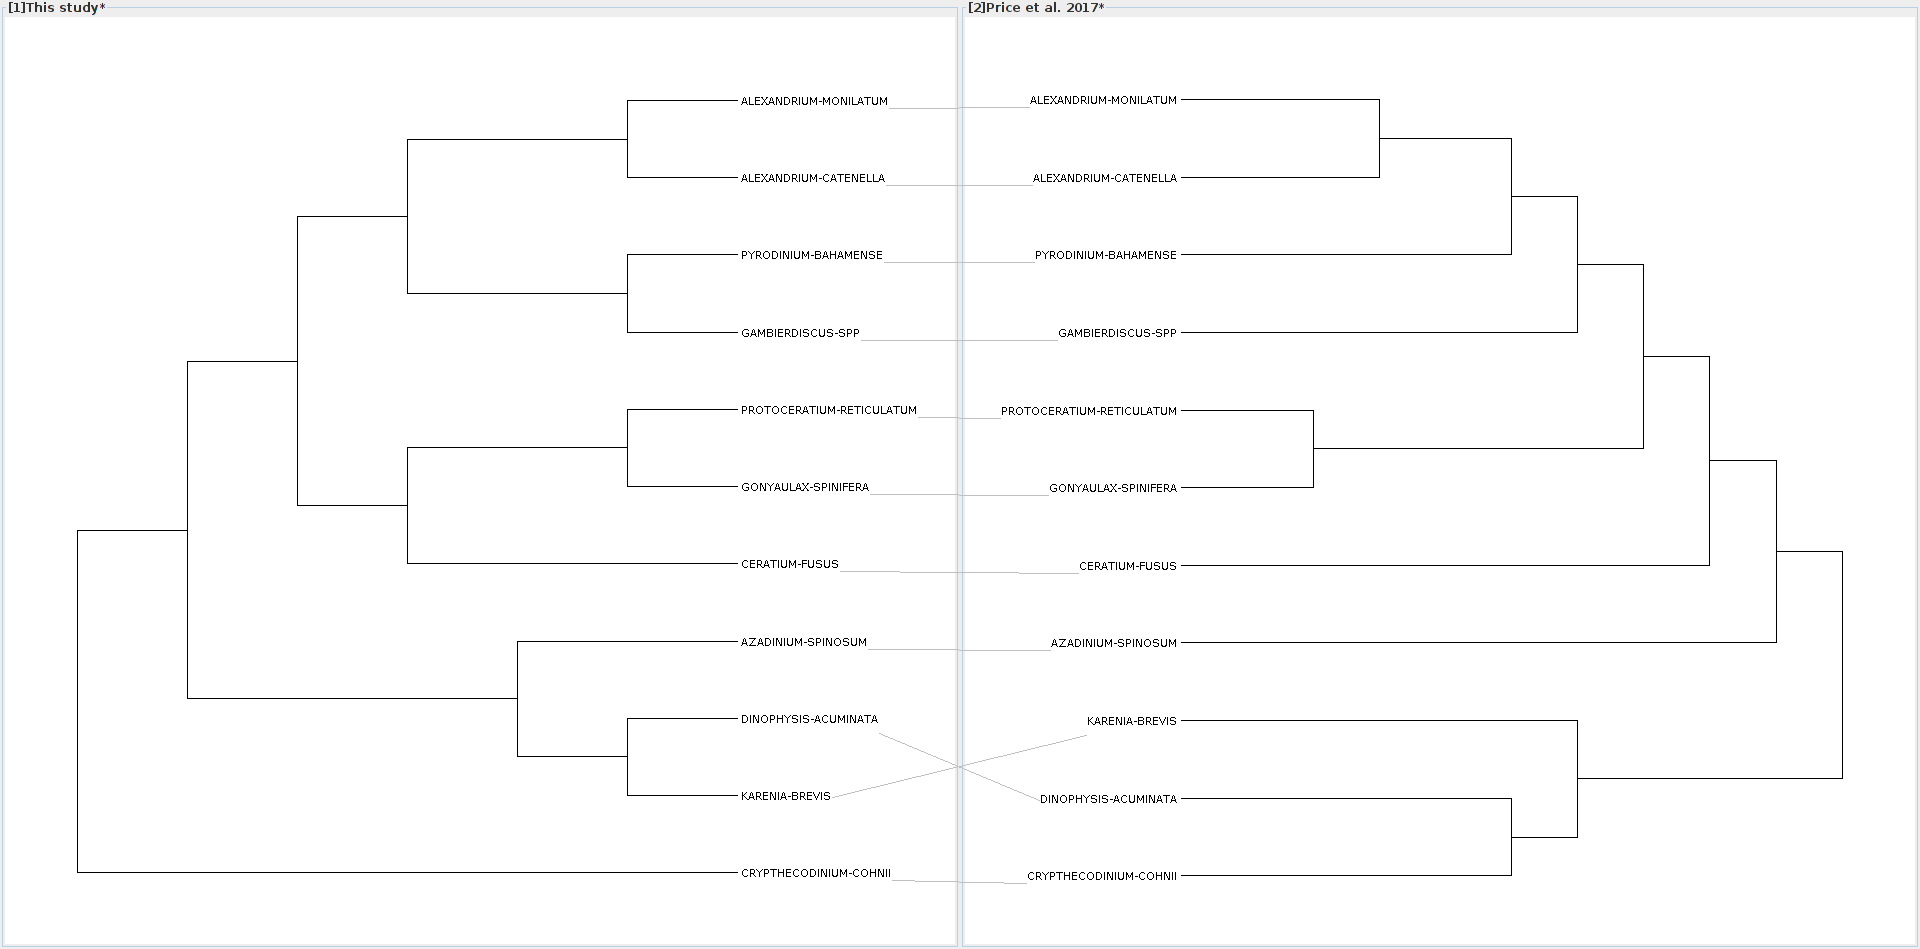
\includegraphics[scale=.23]{Price-comparison.png} 
%\caption{Tanglegram of topology presented in this study (a); and Price et al. (2017) (b). Taxa uncommon to both studies not shown.} 
%\label{fig:tangle}
%\end{figure} 
%\FloatBarrier
In this study, we utilised the BUSCO output which screens for and verifies single copy genes for input into species tree inference, a purpose which was suggested as ideal by the authors of the software \cite{simao2015busco}. 
With adjusting the RNA-seq library trimming values and assembly methods to what we understand to be best practice, and then stringently and transparently selecting single copy genes, the authors believe to have addressed common methodological issues for phylogenetic inference with due diligence. 


\subsection*{Comparison of models tested in this study} 
Once the quality of the transcriptome assembly and gene selection for comparison is satisfied, the next question concerns the adequacy of the models used as a proxy for the evolutionary inference. 
%TODO up to here
\subsubsection*{Inferring species evolution from a small subset of genes such as ribosomal genes, whose evolution may not reflect that of the species.}
\FloatBarrier 
% Alveolates rDNA copies some of the highest extreme long branch content \cite{he2016reducing}
%\cite{ochieng2007nuclear}  don't even know if this is any good but has rdna of eucalypts
Using LSU or SSU rDNA regions for phylogenetics is common practice, at times supplemented with a small number of other genes \cite{shalchian2006combined,zhang2007three,saldarriaga2004molecular,murray2005improving,hoppenrath2010dinoflagellate} 
It is important to acknowledge that these represent the evolutionary history of highly conserved genes, which does not necessarily represent the species evolution. 
Hence studies which utilise primarily rDNA genes for inferring species phylogeny run the risk of presenting the evolutionary history of rDNA genes as synonymous with species evolution when they are in fact poor representatives of the evolutionary history of the majority of nuclear genes?
To address this obstacle, a range of genes need to be used to infer the species evolution.

\begin{figure} 
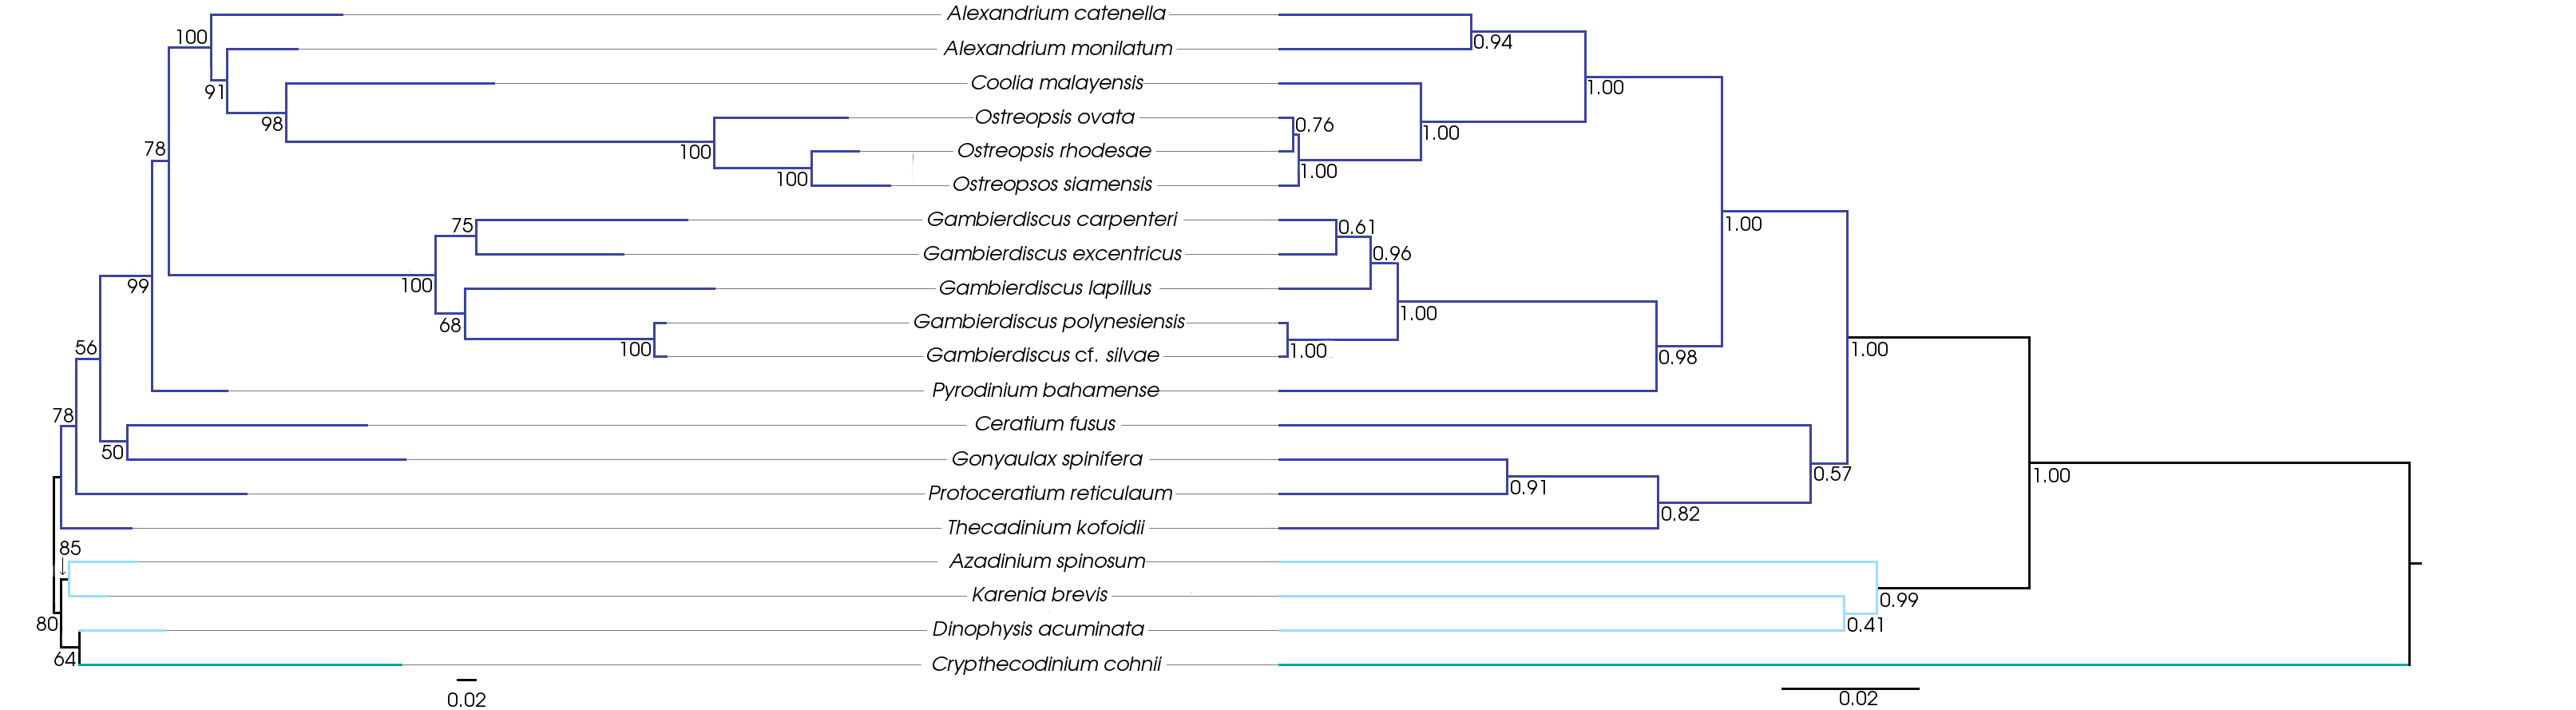
\includegraphics[scale=.2]{figures/MSC-BI_vs_rDNA-ML.png} 
\caption{Tanglegram showing the topological differences in phylogenies from (A) MSC starbeast inference with 58 single copy genes; and (B) concatenated rDNA genes (SSU and D1-D3 LSU)infered with ML. 
Gonyaulacales (\#16) in purple, outgroups (\#3) in light blue and taxa \textit{incertae sedis} (\#1) in teal.} 
\label{fig:tanglerDNA}
\end{figure} 
\FloatBarrier

\subsubsection*{Concatenating selected genes and using ML methods for species inference.}
\FloatBarrier
% Disagreements in deeper branches in insect phylogenomic study which compared models - but used concat \cite{boussau2014strepsiptera}
Concatenation of genes coupled with running ML inference is a commonly used method as it is computationally cheap in comparison to BI methods. 
However as demonstrated by Kubatko et al. (2007) and Roche et al. (2015), this approach is error prone and can be misleading by presenting high bootstrap values on incorrect clades which is positively misleading.
The application of concatenation in combination with ML is common practice in phylogenetic studies for gonyaulacoids  \cite{shalchian2006combined,zhang2007three,saldarriaga2004molecular,murray2005improving,hoppenrath2010dinoflagellate}.
This issue is addressed in this study by running BI under a multi-species coalescence process.
 
\begin{figure} 
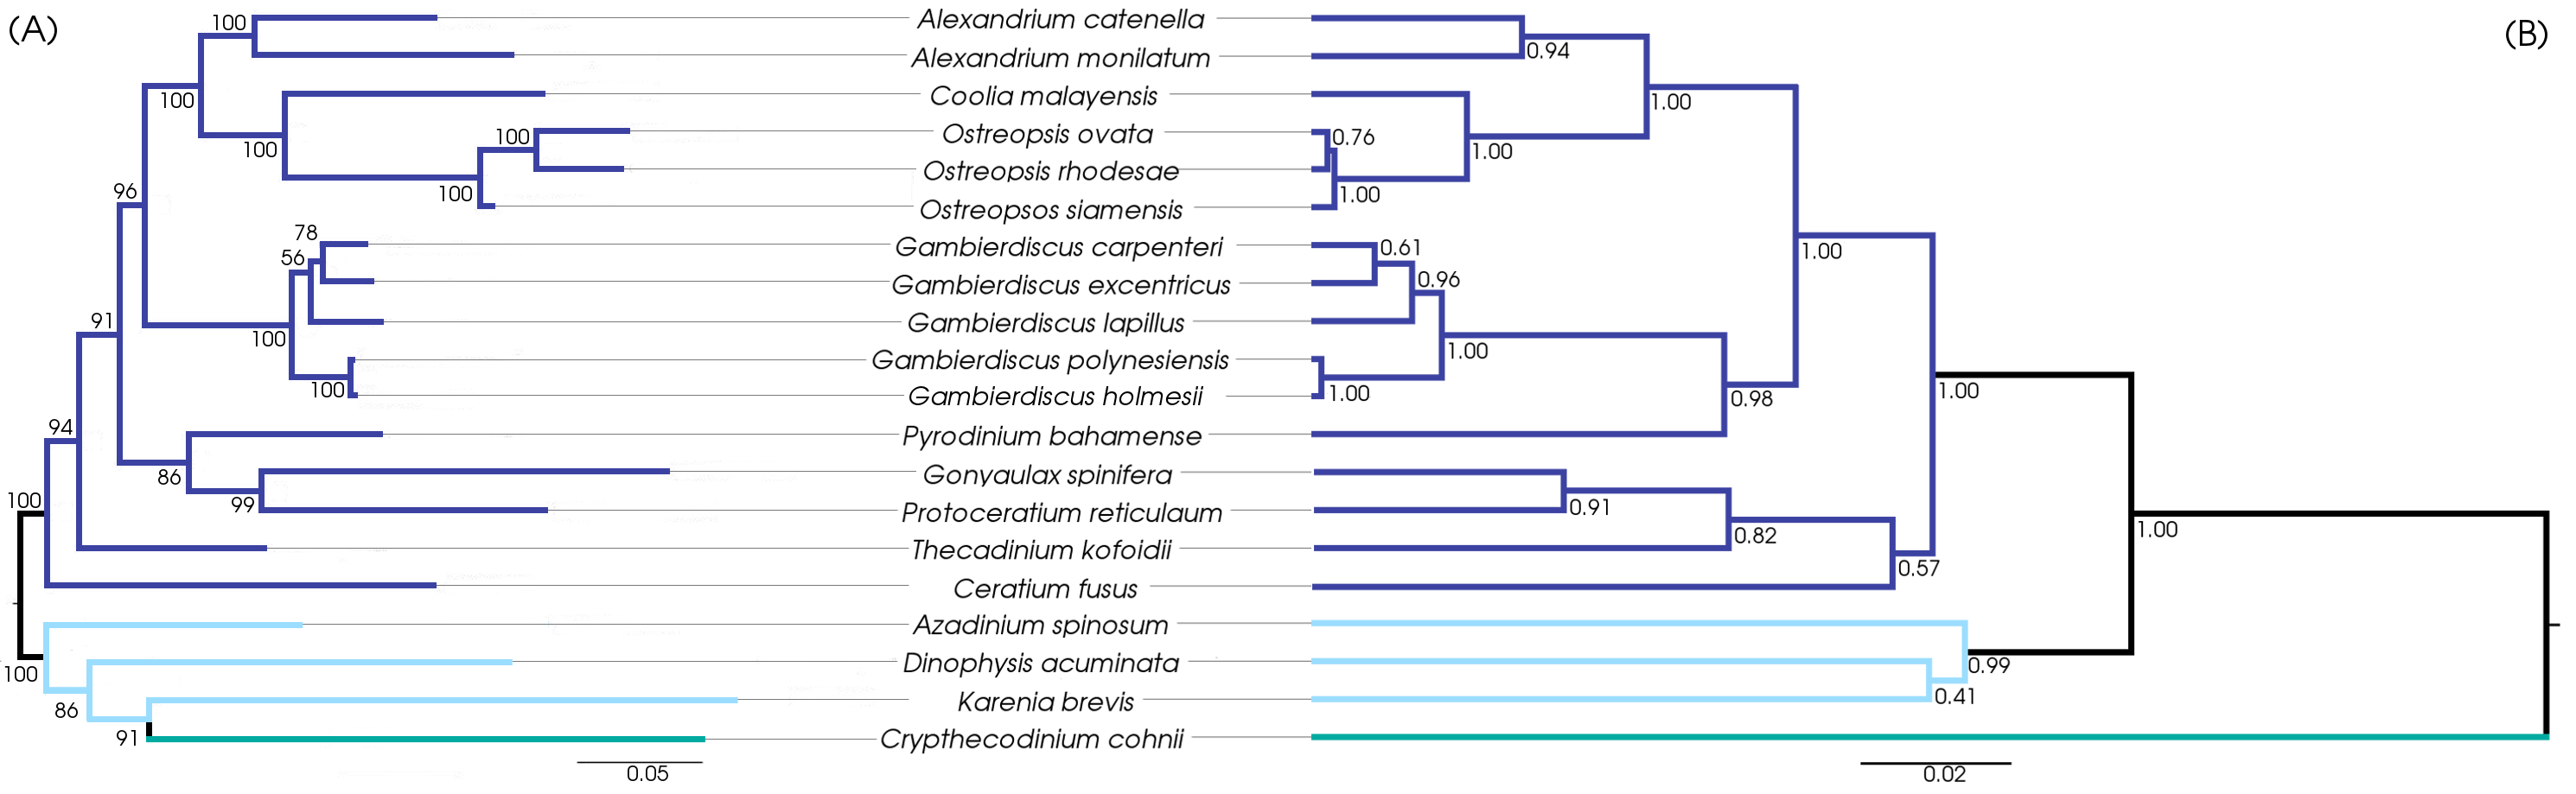
\includegraphics[scale=.2]{figures/MSC-BI_vs_singlecopy-concat-ML.png} 
\caption{Tanglegram showing the topological differences in phylogenies with same 58 single copy gene alignments as input. 
(A) MSC starbeast inference; and (B) concatenated ML inference. 
Gonyaulacales (\#16) in purple, outgroups (\#3) in light blue and taxa \textit{incertae sedis} (\#1) in teal.} 
\label{fig:tangleconcatML}
\end{figure} 
\FloatBarrier

\subsubsection*{Concatenating selected genes and using BI methods for species inference.}
\FloatBarrier 
%Suzuki 2002 shows that PP is overestimated when concatenation is used
%TODO \cite{baele2012accurate} for Path sampling as accurate model assessment method for relaxed clock models... are any improper priors used? PS may not be able to sample from the prior

% MSC robust for both ILS & LBA unlike concat <3 \cite{liu2014coalescent} ; example from water lillies with same phenomenon \cite{liu2014coalescent}

\begin{figure} 
%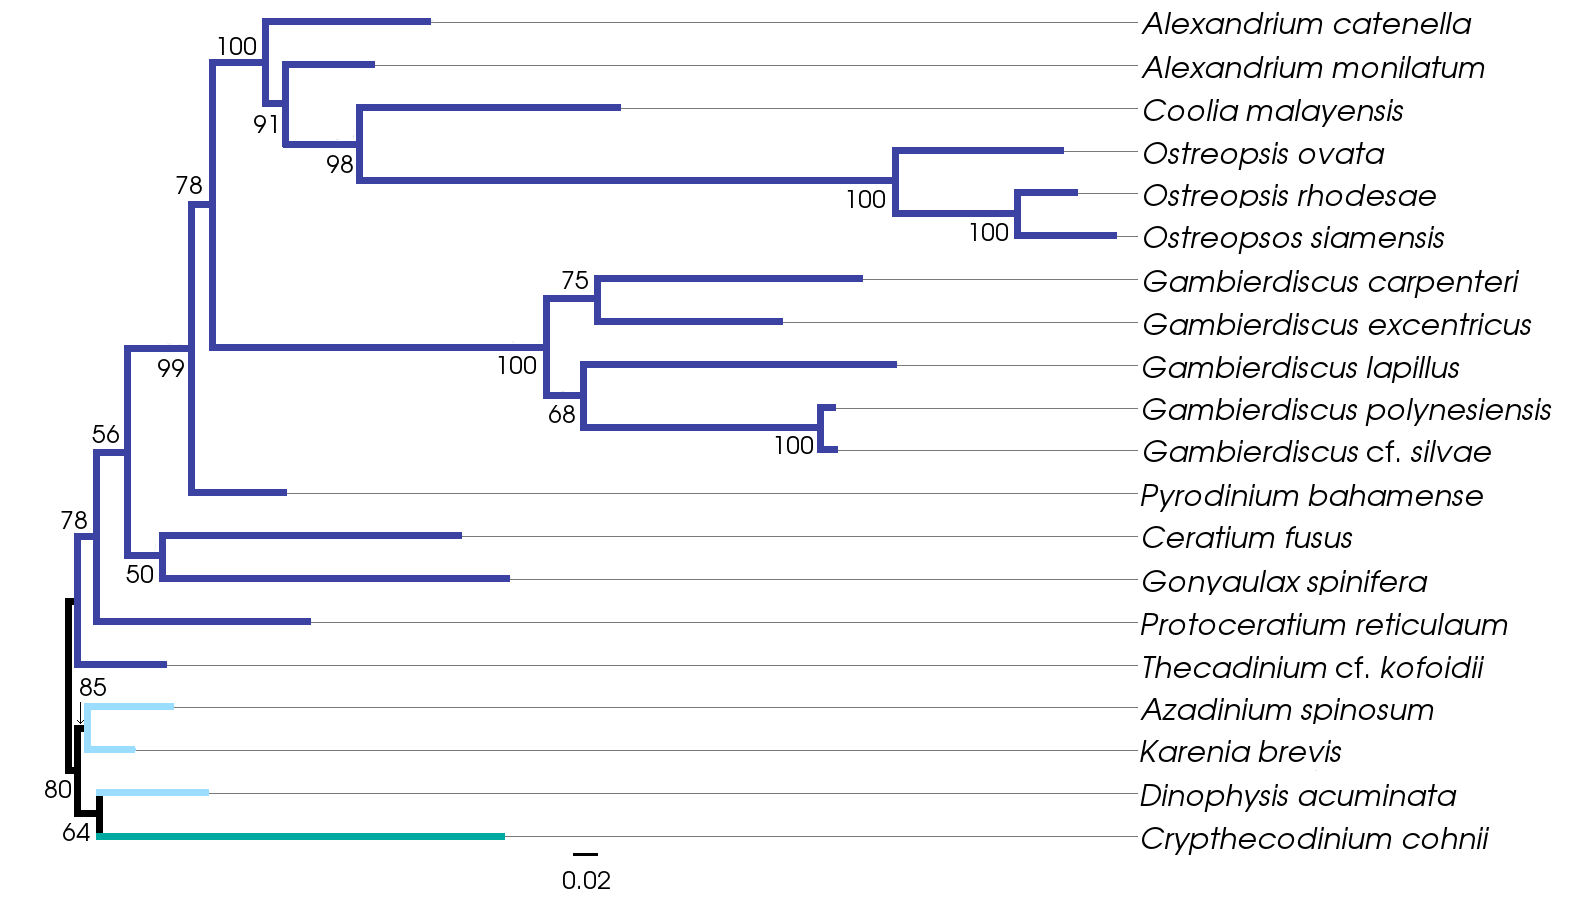
\includegraphics[scale=.23]{figures/rDNA-ML.png} 
\caption{Tanglegram showing the topological differences in phylogenies with same 58 single copy gene alignments as input. 
(A) MSC starbeast inference; and (B) concatenated beast2 inference. 
Gonyaulacales (\#16) in purple, outgroups (\#3) in light blue and taxa \textit{incertae sedis} (\#1) in teal.} 
\label{fig:tangleconcatBI}
\end{figure} 
\FloatBarrier


\subsection*{Limitations of study}
In the previous section we identified potential problems with common approaches to species inference for the gonyaulacales, and then presented a pipeline which attempts to address these problems. 
However we in no way want to imply that this study is not fraught with potential pitfalls too. 
We aim to present avenues for improvement for current methods, especially in areas where large datsets are recently unlocked such as in marine protists with the MMETSP project. %Models and methodology build upon previous work and improve with increased collective knowledge, take the progression for nucleotide substitution rates as an example. The JC69 model from 1969 assumes the substitutions rates between all nuceleotides are equal, including between purines and pyrimidines \cite{}. Through a series of increased complexity to model transition \& transversion rates (i.e. the likelihood of nucleotide change from purine to pyrimidine and vice versa) and steady-state distributions (frequency of each nucleotide given infinite time), the HK85 model was proposed in 1985 \cite{}.
%I may have gone on a tangent here. Probably leave that out.
What follows is the identification of issues with the approach presented in this study, which the authors hope that these will be improved upon in the future. 
%\subsubsection*{Pipeline specific issues}
\paragraph*{Trimming of RNA seq libraries.} The cut off values chosen for this study are based on the recommendations of MacMannes (2014) for optimal transcript discovery. 
However the recommendations are based on an RNA-seq library from mouse embryonic stem cells, which may not be an adequate model for dinoflagellates. 
This could confound the difference between single copy genes and sequencing artifacts.
%\paragraph*{Single copy gene selection bias.} The selection of single copy genes is based on BUSCOv2 hmmer libraries. The pre-screening process by which may have inherent selection bias that is not tranparent to us // Not sure if this one is a problem =/
\paragraph*{Assembly parameters.}
Trinity was chosen as the assembler for this study based on the findings of Honaas et al. (2016), in which Trinity was one of the top performing assemblers for \textit{de novo} transcriptomes as tested with \textit{Arabidopsis thaliana}, a plant with some similar genetic features to dinoflagellates.
Further, Trinity performed well for identifying isoforms of genes and excelled at assembling highly expressed genes \cite{honaas2016selecting}.
Conversely, Cerveau et al. (2016) found that Trinity, CLC Bio and IDBA-Tran assemblies all contain bioinformatic artifacts. 
Using a combination of all three assemblers yielded a final assembly closer to biological reality than any individual assembler, when no reference genome is available \cite{cerveau2016combining}.
As this study uses Trinity exclusively, it is subject to the bioinformatic errors found by Cerveau et al. which could affect downstream analysis.
%\paragraph*{Amino acid substitution model.} WAG model
%\paragraph*{Molecular clock model selection.} Relaxed clock normal
%\subsubsection*{Gonyaulacales specific issues}
\paragraph*{Contamination of other taxa.} 
The 650+ RNA extract submission to MMETSP was from a large number of investigators and low level contamination is inherent in the project \cite{keeling2014marine}. 
As the cultures tested in all the studies contributing to this dataset were not axenic, contamination could be bacterial or eukaryotic in nature and could result in misleading gene phylogenies which were used to infer the species phylogeny.
\paragraph*{No representative genome for comparison.} 
Without a guided genome comparison, it is difficult to extrapolate on the assembly adequacy and whether the genes selected are single copies, or  mis-assemblies of paralogs.
\paragraph*{Different methods for RNA-seq.} 
Three different approaches for RNA-seq library generation were employed for the libraries used in this study, the MMETSP taxa were sequences on HiSeq platform with 50bp inserts; while all other taxa were sequenced on the NextSeq platform with 75bp or 150bp inserts.
\paragraph*{Total evidence}

\newpage
\section{Conclusion}
With the accessibility of large data sets, the focus needs to fall on the methodology for investigating them. 
This study presents a pipeline to process RNA-seq libraries through assembly, single copy gene selection to phylogenetic species inference. 
As a case study, the gonyaulacales phylogeny was elucidated as taxa within this order are rife with paralogs. 
The resulting phylogeny shows a well resolved, well supported inference of the gonyaulacales evolution. 
By presenting the pipeline designed in this study we hope that the use of reproducible, open-access processing of large data-sets such as the MMETSP database becomes the standard.  
\newpage

\section{Acknowledgments}
The GVL section of this study was conducted inside the National eResearch Collaboration Tools and Resources (NeCTAR) research cloud, an initiative by the National Research Infrastructure for Australia (NCRIS).
Gratitude to the Stanley Watson foundation, the Linnaean Society of New South Wales, and the ABRS National Taxonomy Research Student Travel Bursary for funding A. L. Kretzschmar's attendance at the Molecular Evolution workshop at the Marine biological laboratory, Woods Hole, MA, USA.
Shout out to the Taming the BEAST organizers \& fellow attendees for a most illuminating workshop in February 2017 on BEAST methodology, and to Geneious for subsidizing A. L. Kretzschmar's attendance fee.
Thank you to Dr. Tim Kahlke for running Interproscan for transcriptome analysis.
\section{Supplementary material}
\FloatBarrier
\begin{table}
\caption{Table S1: Culturing conditions for species processed for this study.}
%\label{tbl:strainTable}
\begin{tabular}{ | p{3cm} | p{2.5cm} | p{1.5cm} | p{5.3cm} |}
\hline
\textbf{Species} & \textbf{Strain}& \textbf{Temp} & \textbf{Source location} \\
%\hline
%\textit{Coolia malayensis}&MAB&& \\
\hline
\textit{Gambierdiscus carpenteri}&UTSMER9A&17&Merimbula, AU\\
\hline
\textit{Gambierdiscus lapillus}&HG4&27&Heron Island, AU\\
\hline
\textit{Gambierdiscus polynesiensis}&CG15&27&Rarotonga, COK\\
\hline
\textit{Gambierdiscus} cf. \textit{silvae}&HG5&27&Heron Island, AU\\
\hline
%\textit{Ostreopsis ovata}&HER27&&\\
%\hline
%\textit{Ostreopsis rhodesae}&HER26&&\\
%\hline
%\textit{Ostreopsis siamensis}&BH1&&\\
%\hline
\textit{Thecadinium} cf. \emph{kofoidii}&THECA&18&Gordons bay, Sydney, AU\\
\hline
\end{tabular}
\end{table}
\FloatBarrier

\begin{longtable}{  | p{3.5cm} |p{2.2cm} | p{1.8cm} | p{1.8cm} | p{1.8cm} | p{3cm} |}
\caption{Table S2: Transcriptomes used for study along including strain ID, source and BUSCOv2 information. MMETSP abbreviation for marine Microbial eukaryotic transcriptome sequencing project, by Moore Foundation.}\\
\hline
%\label{tbl:Transcriptomes}
%\textbf{Family}&
\textbf{Species}&\textbf{Strain}&\textbf{complete BUSCOs}&\textbf{single complete BUSCOs}&\textbf{fragmented BUSCOs}&\textbf{Source}\\
\hline
 \multicolumn{6}{| c |}{Gonyaulacales transcriptomes}\\
    \hline
\emph{Alexandrium catenella}&OF101&110&74&3&MMETSP0790 \citep{keeling2014marine}\\
        \hline
\emph{Alexandrium monilatum}&JR08&107&74&3&MMETSP0093 \citep{keeling2014marine}\\
        \hline
\emph{Ceratium fusus}&PA161109&121&81&4&MMETSP1074 \citep{keeling2014marine}\\
        \hline
\emph{Coolia malayensis}&MAB&138&100&1&(Verma 2018, in prep)\\
\hline
\emph{Crypthecodinium cohnii}&Seligo&126&98&0&MMETSP0326\_2 \citep{keeling2014marine}\\
        \hline
\emph{Gambierdiscus carpenteri}&UTSMER9A&101&83&2&This study\\
\hline
\emph{Gambierdiscus excentricus}&VGO790&88&83&4&\cite{kohli2017role}\\
        \hline
\emph{Gambierdiscus lapillus}&HG4&141&98&2&This study\\
        \hline
\emph{Gambierdiscus polynesiensis}&CG15&104&81&3&This study\\
        \hline
\emph{Gambierdiscus} cf. \emph{silvae}&HG5&134&87&2&This study\\
        \hline
\emph{Gonyaulax spinifera}&CCMP409&83&53&2&MMETSP1439 \citep{keeling2014marine}\\
        \hline
\emph{Ostreopsis ovata}&HER27&132&99&2&(Verma 2018, in prep)\\
     \hline
\emph{Ostreopsis rhodesae}&HER26&131&98&1&(Verma 2018, in prep)\\
     \hline
\emph{Ostreopsis siamensis}&BH1&132&98&1&(Verma 2018, in prep)\\
     \hline
\emph{Protoceratium reticulatum}&CCCM535=CCMP1889&108&72&5&MMETSP0228 \citep{keeling2014marine}\\
    \hline
\emph{Pyrodinium bahamense}&pbaha01&119&897&2&MMETSP0796 \citep{keeling2014marine}\\
        \hline
\emph{Thecadinium} cf. \emph{kofoidii}&THECA&93&70&5&This study\\
 \hline
 \multicolumn{6}{| c |}{Outgroup transcriptomes}\\
 \hline
 \emph{Azadinium spinosum}&3D9&1.8&81&4&MMETSP1036\_2 \citep{keeling2014marine}\\
        \hline
\emph{Dinophysis acimunata}&DAEP01&117&74&2&MMETSP0797 \citep{keeling2014marine}\\
        \hline
\emph{Karenia brevis}&CCMP2229&115&85&2&MMETSP0030 \citep{keeling2014marine}\\
    \hline
\end{longtable}
\FloatBarrier
%families, sections which was taken out:Ceratiaceae,Crypthecodiniaceae,Gonyaulacaceae,Protoceratiaceae,Dinophysiaceae,Dinophyceae incertae sedis,Gymnodiniales

\begin{longtable}{  | p{3cm} |p{3cm} |  p{3cm} | }
\caption{Table S3: Accession numbers for ribosomal DNA sequences used for Fig. ~\ref{fig:rdna}. Sequences sourced from NCBI, except accesion numbers with '$\ast$' sourced from the Silva database. Genes not publically available are denoted by '-'.}\\
\hline
%\label{tbl:Transcriptomes}
%\textbf{Family}&
\textbf{Species}&\textbf{SSU seq.}&\textbf{D1-D3 LSU seq.}\\

\hline
 \multicolumn{3}{| c |}{Gonyaulacales taxa}\\
 \hline
\emph{Alexandrium catenella}&AB088286&AB088238\\
        \hline
\emph{Alexandrium monilatum}&AY883005&-\\
        \hline
\emph{Ceratium fusus}&AF022153&AF260390\\
        \hline
\emph{Coolia malayensis}&HQ897279$\ast$&KX589143\\
\hline
\emph{Crypthecodinium cohnii}&M64245&-\\
        \hline
\emph{Gambierdiscus carpenteri}&EF202908&EF202938\\
\hline
\emph{Gambierdiscus excentricus}&GETL01000157$\ast$&HQ877874\\
        \hline
\emph{Gambierdiscus lapillus}&KU558930&-\\
        \hline
\emph{Gambierdiscus polynesiensis}&EF202907&This study\\
        \hline
\emph{Gambierdiscus} cf. \emph{silvae}&This study&this study\\
        \hline
\emph{Gonyaulax spinifera}&AF022155&DQ151558\\
        \hline
\emph{Ostreopsis ovata}&AF244939&KJ781420\\
     \hline
\emph{Ostreopsis rhodesae}&KX055855&KX055845\\
     \hline
\emph{Ostreopsis siamensis}&KX055868&HQ414223\\
     \hline
\emph{Protoceratium reticulatum}&AF274273&EF613362\\
    \hline
\emph{Pyrodinium bahamense}&AY456115&AB936757\\
        \hline
\emph{Thecadinium} cf. \emph{kofoidii}&AY238478&KT371445\\
 \hline
\multicolumn{3}{| c |}{Outgroup taxa}\\
    \hline
  \emph{Azadinium spinosum}&JN680857&JN165101\\
        \hline
\emph{Dinophysis acimunata}&AJ506972&EF613351\\
        \hline
\emph{Karenia brevis}&EF492504&AY355458\\
\hline
\end{longtable}
\FloatBarrier

\newpage
\bibliographystyle{acm}
\bibliography{gonya.bib}


\end{document}